%\SweaveUTF8
\documentclass[aspectratio=169]{beamer}

\usetheme{default}
% Slide setup, colour independent

\usepackage{amsmath,amssymb,amsthm}
\usepackage[utf8]{inputenc}
\usepackage{colortbl}
\usepackage{bm}
\usepackage{xcolor}
\usepackage{dsfont}
\usepackage{setspace}
%\usepackage{subfigure}
% To use \ding{234} and the like
\usepackage{pifont}
% To cross reference between slide files
\usepackage{zref-xr,zref-user}
% Use something like
% \zexternaldocument{fileI}
% in the tex files. And cite using \zref instead of \ref

% Fields and the like
\def\IC{\mathbb{C}}
\def\IF{\mathbb{F}}
\def\II{\mathbb{I}}
\def\IJ{\mathbb{J}}
\def\IM{\mathbb{M}}
\def\IN{\mathbb{N}}
\def\IP{\mathbb{P}}
\def\IR{\mathbb{R}}
\def\IZ{\mathbb{Z}}
\def\11{\mathds{1}}


% Bold lowercase
\def\ba{\bm{a}}
\def\bb{\bm{b}}
\def\bc{\bm{c}}
\def\bd{\bm{d}}
\def\be{\bm{e}}
\def\bf{\bm{f}}
\def\bh{\bm{h}}
\def\bi{\bm{i}}
\def\bj{\bm{j}}
\def\bk{\bm{k}}
\def\bn{\bm{n}}
\def\bp{\bm{p}}
\def\br{\bm{r}}
\def\bs{\bm{s}}
\def\bu{\bm{u}}
\def\bv{\bm{v}}
\def\bw{\bm{w}}
\def\bx{\bm{x}}
\def\by{\bm{y}}
\def\bz{\bm{z}}

% Bold capitals
\def\bB{\bm{B}}
\def\bD{\bm{D}}
\def\bE{\bm{E}}
\def\bF{\bm{F}}
\def\bG{\bm{G}}
\def\bI{\bm{I}}
\def\bL{\bm{L}}
\def\bN{\bm{N}}
\def\bP{\bm{P}}
\def\bR{\bm{R}}
\def\bS{\bm{S}}
\def\bT{\bm{T}}
\def\bX{\bm{X}}

% Bold numbers
\def\b0{\bm{0}}

% Bold greek
\bmdefine{\bmu}{\bm{\mu}}
\def\bphi{\bm{\phi}}
\def\bvarphi{\bm{\varphi}}
\def\bPi{\bm{\Pi}}
\def\bGamma{\bm{\Gamma}}

% Bold red sentence
\def\boldred#1{{\color{red}\textbf{#1}}}
\def\defword#1{{\color{orange}\textbf{#1}}}

% Caligraphic letters
\def\A{\mathcal{A}}
\def\B{\mathcal{B}}
\def\C{\mathcal{C}}
\def\D{\mathcal{D}}
\def\E{\mathcal{E}}
\def\F{\mathcal{F}}
\def\G{\mathcal{G}}
\def\H{\mathcal{H}}
\def\I{\mathcal{I}}
\def\L{\mathcal{L}}
\def\M{\mathcal{M}}
\def\N{\mathcal{N}}
\def\P{\mathcal{P}}
\def\R{\mathcal{R}}
\def\S{\mathcal{S}}
\def\T{\mathcal{T}}
\def\U{\mathcal{U}}
\def\V{\mathcal{V}}

% Adding space for prime (') where needed
\def\pprime{\,'}
% Adding space for star (\star) where needed
\def\pstar{{\,\star}}

% tt font for code
\def\code#1{{\tt #1}}

% i.e., e.g.
\def\eg{\emph{e.g.}}
\def\ie{\emph{i.e.}}


% Operators and special symbols
\def\nbOne{{\mathchoice {\rm 1\mskip-4mu l} {\rm 1\mskip-4mu l}
{\rm 1\mskip-4.5mu l} {\rm 1\mskip-5mu l}}}
\def\cov{\ensuremath{\mathsf{cov}}}
\def\Var{\ensuremath{\mathsf{Var}\ }}
\def\Im{\textrm{Im}\;}
\def\Re{\textrm{Re}\;}
\def\det{\ensuremath{\mathsf{det}}}
\def\diag{\ensuremath{\mathsf{diag}}}
\def\nullspace{\ensuremath{\mathsf{null}}}
\def\nullity{\ensuremath{\mathsf{nullity}}}
\def\rank{\ensuremath{\mathsf{rank}}}
\def\range{\ensuremath{\mathsf{range}}}
\def\sgn{\ensuremath{\mathsf{sgn}}}
\def\Span{\ensuremath{\mathsf{span}}}
\def\tr{\ensuremath{\mathsf{tr}}}
\def\imply{$\Rightarrow$}
\def\restrictTo#1#2{\left.#1\right|_{#2}}
\newcommand{\parallelsum}{\mathbin{\!/\mkern-5mu/\!}}
\def\dsum{\mathop{\displaystyle \sum }}%
\def\dind#1#2{_{\substack{#1\\ #2}}}

\DeclareMathOperator{\GL}{GL}
\DeclareMathOperator{\Rel}{Re}
\def\Nt#1{\left|\!\left|\!\left|#1\right|\!\right|\!\right|}
\newcommand{\tripbar}{|\! |\! |}



% The beamer bullet (in base colour)
\def\bbullet{\leavevmode\usebeamertemplate{itemize item}\ }

% Theorems and the like
\newtheorem{proposition}[theorem]{Proposition}
\newtheorem{property}[theorem]{Property}
\newtheorem{importantproperty}[theorem]{Property}
\newtheorem{importanttheorem}[theorem]{Theorem}
%\newtheorem{lemma}[theorem]{Lemma}
%\newtheorem{corollary}[theorem]{Corollary}
\newtheorem{remark}[theorem]{Remark}
\setbeamertemplate{theorems}[numbered]
%\setbeamertemplate{theorems}[ams style]

%
%\usecolortheme{orchid}
%\usecolortheme{orchid}

\def\red{\color[rgb]{1,0,0}}
\def\blue{\color[rgb]{0,0,1}}
\def\green{\color[rgb]{0,1,0}}


% Get rid of navigation stuff
\setbeamertemplate{navigation symbols}{}

% Set footline/header line
\setbeamertemplate{footline}
{%
\quad p. \insertpagenumber \quad--\quad \insertsection\vskip2pt
}
% \setbeamertemplate{headline}
% {%
% \quad\insertsection\hfill p. \insertpagenumber\quad\mbox{}\vskip2pt
% }


\makeatletter
\newlength\beamerleftmargin
\setlength\beamerleftmargin{\Gm@lmargin}
\makeatother

% Colours for special pages
\def\extraContent{yellow!20}


%%%%%%%%%%%%%%%%%
\usepackage{tikz}
\usetikzlibrary{shapes,arrows}
\usetikzlibrary{positioning}
\usetikzlibrary{shapes.symbols,shapes.callouts,patterns}
\usetikzlibrary{calc,fit}
\usetikzlibrary{backgrounds}
\usetikzlibrary{decorations.pathmorphing,fit,petri}
\usetikzlibrary{automata}
\usetikzlibrary{fadings}
\usetikzlibrary{patterns,hobby}
\usetikzlibrary{backgrounds,fit,petri}


\usepackage{pgfplots}
\pgfplotsset{compat=1.6}
\pgfplotsset{ticks=none}

\usetikzlibrary{decorations.markings}
\usetikzlibrary{arrows.meta}
\tikzset{>=stealth}

% For tikz
\tikzstyle{cloud} = [draw, ellipse,fill=red!20, node distance=0.87cm,
minimum height=2em]
\tikzstyle{line} = [draw, -latex']


%%% For max frame images
\newenvironment{changemargin}[2]{%
\begin{list}{}{%
\setlength{\topsep}{0pt}%
\setlength{\leftmargin}{#1}%
\setlength{\rightmargin}{#2}%
\setlength{\listparindent}{\parindent}%
\setlength{\itemindent}{\parindent}%
\setlength{\parsep}{\parskip}%
}%
\item[]}{\end{list}}


% Make one image take up the entire slide content area in beamer,.:
% centered/centred full-screen image, with title:
% This uses the whole screen except for the 1cm border around it
% all. 128x96mm
\newcommand{\titledFrameImage}[2]{
\begin{frame}{#1}
%\begin{changemargin}{-1cm}{-1cm}
\begin{center}
\includegraphics[width=108mm,height=\textheight,keepaspectratio]{#2}
\end{center}
%\end{changemargin}
\end{frame}
}

% Make one image take up the entire slide content area in beamer.:
% centered/centred full-screen image, no title:
% This uses the whole screen except for the 1cm border around it
% all. 128x96mm
\newcommand{\plainFrameImage}[1]{
\begin{frame}[plain]
%\begin{changemargin}{-1cm}{-1cm}
\begin{center}
\includegraphics[width=108mm,height=76mm,keepaspectratio]{#1}
\end{center}
%\end{changemargin}
\end{frame}
}

% Make one image take up the entire slide area, including borders, in beamer.:
% centered/centred full-screen image, no title:
% This uses the entire whole screen
\newcommand{\maxFrameImage}[1]{
\begin{frame}[plain]
\begin{changemargin}{-1cm}{-1cm}
\begin{center}
\includegraphics[width=\paperwidth,height=\paperheight,keepaspectratio]
{#1}
\end{center}
\end{changemargin}
\end{frame}
}

% This uses the entire whole screen (to include in frame)
\newcommand{\maxFrameImageNoFrame}[1]{
\begin{changemargin}{-1cm}{-1cm}
\begin{center}
\includegraphics[width=\paperwidth,height=0.99\paperheight,keepaspectratio]
{#1}
\end{center}
\end{changemargin}
}

% Make one image take up the entire slide area, including borders, in beamer.:
% centered/centred full-screen image, no title:
% This uses the entire whole screen
\newcommand{\maxFrameImageColor}[2]{
\begin{frame}[plain]
\setbeamercolor{normal text}{bg=#2!20}
\begin{changemargin}{-1cm}{-1cm}
\begin{center}
\includegraphics[width=\paperwidth,height=\paperheight,keepaspectratio]
{#1}
\end{center}
\end{changemargin}
\end{frame}
}


\usepackage{tikz}
\usetikzlibrary{patterns,hobby}
\usepackage{pgfplots}
\pgfplotsset{compat=1.6}
\pgfplotsset{ticks=none}

\usetikzlibrary{backgrounds}
\usetikzlibrary{decorations.markings}
\usetikzlibrary{arrows.meta}
\tikzset{>=stealth}

\tikzset{
  clockwise arrows/.style={
    postaction={
      decorate,
      decoration={
        markings,
        mark=between positions 0.1 and 0.9 step 40pt with {\arrow{>}},
   }}}}


   %%%%%%%%%%%
% To have links to parts in the outline
\makeatletter
\AtBeginPart{%
  \addtocontents{toc}{\protect\beamer@partintoc{\the\c@part}{\beamer@partnameshort}{\the\c@page}}%
}
%% number, shortname, page.
\providecommand\beamer@partintoc[3]{%
  \ifnum\c@tocdepth=-1\relax
    % requesting onlyparts.
    \makebox[6em]{Part #1:} \textcolor{green!30!blue}{\hyperlink{#2}{#2}}
    \par
  \fi
}
\define@key{beamertoc}{onlyparts}[]{%
  \c@tocdepth=-1\relax
}
\makeatother%

\newcommand{\nameofthepart}{}
\newcommand{\nupart}[1]%
    {   \part{#1}%
        \renewcommand{\nameofthepart}{#1}%
        {
          \setbeamercolor{background canvas}{bg=orange!50}
          \begin{frame}{#1}%\partpage 
          \hypertarget{\nameofthepart}{}\tableofcontents%
          \end{frame}
        }
    }



\usecolortheme{orchid}
%% Listings
\usepackage{listings}
\definecolor{mygreen}{rgb}{0,0.6,0}
\definecolor{mygray}{rgb}{0.5,0.5,0.5}
\definecolor{mymauve}{rgb}{0.58,0,0.82}
\definecolor{mygold}{rgb}{1,0.843,0}
\definecolor{myblue}{rgb}{0.537,0.812,0.941}

\definecolor{lgreen}{rgb}{0.6,0.9,.6}
\definecolor{lred}{rgb}{1,0.5,.5}

\lstloadlanguages{R}
\lstset{ %
  language=R,
  backgroundcolor=\color{black!05},   % choose the background color
  basicstyle=\footnotesize\ttfamily,        % size of fonts used for the code
  breaklines=true,                 % automatic line breaking only at whitespace
  captionpos=b,                    % sets the caption-position to bottom
  commentstyle=\color{mygreen},    % comment style
  escapeinside={\%*}{*)},          % if you want to add LaTeX within your code
  keywordstyle=\color{red},       % keyword style
  stringstyle=\color{mygold},     % string literal style
  keepspaces=true,
  columns=fullflexible,
  tabsize=4,
}
% Could also do (in lstset)
% basicstyle==\fontfamily{pcr}\footnotesize
\lstdefinelanguage{Renhanced}%
  {keywords={abbreviate,abline,abs,acos,acosh,action,add1,add,%
      aggregate,alias,Alias,alist,all,anova,any,aov,aperm,append,apply,%
      approx,approxfun,apropos,Arg,args,array,arrows,as,asin,asinh,%
      atan,atan2,atanh,attach,attr,attributes,autoload,autoloader,ave,%
      axis,backsolve,barplot,basename,besselI,besselJ,besselK,besselY,%
      beta,binomial,body,box,boxplot,break,browser,bug,builtins,bxp,by,%
      c,C,call,Call,case,cat,category,cbind,ceiling,character,char,%
      charmatch,check,chol,chol2inv,choose,chull,class,close,cm,codes,%
      coef,coefficients,co,col,colnames,colors,colours,commandArgs,%
      comment,complete,complex,conflicts,Conj,contents,contour,%
      contrasts,contr,control,helmert,contrib,convolve,cooks,coords,%
      distance,coplot,cor,cos,cosh,count,fields,cov,covratio,wt,CRAN,%
      create,crossprod,cummax,cummin,cumprod,cumsum,curve,cut,cycle,D,%
      data,dataentry,date,dbeta,dbinom,dcauchy,dchisq,de,debug,%
      debugger,Defunct,default,delay,delete,deltat,demo,de,density,%
      deparse,dependencies,Deprecated,deriv,description,detach,%
      dev2bitmap,dev,cur,deviance,off,prev,,dexp,df,dfbetas,dffits,%
      dgamma,dgeom,dget,dhyper,diag,diff,digamma,dim,dimnames,dir,%
      dirname,dlnorm,dlogis,dnbinom,dnchisq,dnorm,do,dotplot,double,%
      download,dpois,dput,drop,drop1,dsignrank,dt,dummy,dump,dunif,%
      duplicated,dweibull,dwilcox,dyn,edit,eff,effects,eigen,else,%
      emacs,end,environment,env,erase,eval,equal,evalq,example,exists,%
      exit,exp,expand,expression,External,extract,extractAIC,factor,%
      fail,family,fft,file,filled,find,fitted,fivenum,fix,floor,for,%
      For,formals,format,formatC,formula,Fortran,forwardsolve,frame,%
      frequency,ftable,ftable2table,function,gamma,Gamma,gammaCody,%
      gaussian,gc,gcinfo,gctorture,get,getenv,geterrmessage,getOption,%
      getwd,gl,glm,globalenv,gnome,GNOME,graphics,gray,grep,grey,grid,%
      gsub,hasTsp,hat,heat,help,hist,home,hsv,httpclient,I,identify,if,%
      ifelse,Im,image,\%in\%,index,influence,measures,inherits,install,%
      installed,integer,interaction,interactive,Internal,intersect,%
      inverse,invisible,IQR,is,jitter,kappa,kronecker,labels,lapply,%
      layout,lbeta,lchoose,lcm,legend,length,levels,lgamma,library,%
      licence,license,lines,list,lm,load,local,locator,log,log10,log1p,%
      log2,logical,loglin,lower,lowess,ls,lsfit,lsf,ls,machine,Machine,%
      mad,mahalanobis,make,link,margin,match,Math,matlines,mat,matplot,%
      matpoints,matrix,max,mean,median,memory,menu,merge,methods,min,%
      missing,Mod,mode,model,response,mosaicplot,mtext,mvfft,na,nan,%
      names,omit,nargs,nchar,ncol,NCOL,new,next,NextMethod,nextn,%
      nlevels,nlm,noquote,NotYetImplemented,NotYetUsed,nrow,NROW,null,%
      numeric,\%o\%,objects,offset,old,on,Ops,optim,optimise,optimize,%
      options,or,order,ordered,outer,package,packages,page,pairlist,%
      pairs,palette,panel,par,parent,parse,paste,path,pbeta,pbinom,%
      pcauchy,pchisq,pentagamma,persp,pexp,pf,pgamma,pgeom,phyper,pico,%
      pictex,piechart,Platform,plnorm,plogis,plot,pmatch,pmax,pmin,%
      pnbinom,pnchisq,pnorm,points,poisson,poly,polygon,polyroot,pos,%
      postscript,power,ppoints,ppois,predict,preplot,pretty,Primitive,%
      print,prmatrix,proc,prod,profile,proj,prompt,prop,provide,%
      psignrank,ps,pt,ptukey,punif,pweibull,pwilcox,q,qbeta,qbinom,%
      qcauchy,qchisq,qexp,qf,qgamma,qgeom,qhyper,qlnorm,qlogis,qnbinom,%
      qnchisq,qnorm,qpois,qqline,qqnorm,qqplot,qr,Q,qty,qy,qsignrank,%
      qt,qtukey,quantile,quasi,quit,qunif,quote,qweibull,qwilcox,%
      rainbow,range,rank,rbeta,rbind,rbinom,rcauchy,rchisq,Re,read,csv,%
      csv2,fwf,readline,socket,real,Recall,rect,reformulate,regexpr,%
      relevel,remove,rep,repeat,replace,replications,report,require,%
      resid,residuals,restart,return,rev,rexp,rf,rgamma,rgb,rgeom,R,%
      rhyper,rle,rlnorm,rlogis,rm,rnbinom,RNGkind,rnorm,round,row,%
      rownames,rowsum,rpois,rsignrank,rstandard,rstudent,rt,rug,runif,%
      rweibull,rwilcox,sample,sapply,save,scale,scan,scan,screen,sd,se,%
      search,searchpaths,segments,seq,sequence,setdiff,setequal,set,%
      setwd,show,sign,signif,sin,single,sinh,sink,solve,sort,source,%
      spline,splinefun,split,sqrt,stars,start,stat,stem,step,stop,%
      storage,strstrheight,stripplot,strsplit,structure,strwidth,sub,%
      subset,substitute,substr,substring,sum,summary,sunflowerplot,svd,%
      sweep,switch,symbol,symbols,symnum,sys,status,system,t,table,%
      tabulate,tan,tanh,tapply,tempfile,terms,terrain,tetragamma,text,%
      time,title,topo,trace,traceback,transform,tri,trigamma,trunc,try,%
      ts,tsp,typeof,unclass,undebug,undoc,union,unique,uniroot,unix,%
      unlink,unlist,unname,untrace,update,upper,url,UseMethod,var,%
      variable,vector,Version,vi,warning,warnings,weighted,weights,%
      which,while,window,write,\%x\%,x11,X11,xedit,xemacs,xinch,xor,%
      xpdrows,xy,xyinch,yinch,zapsmall,zip},%
   otherkeywords={!,!=,~,$,*,\%,\&,\%/\%,\%*\%,\%\%,<-,<<-,_,/},%
   alsoother={._$},%
   sensitive,%
   morecomment=[l]\#,%
   morestring=[d]",%
   morestring=[d]'% 2001 Robert Denham
  }%

%%%%%%% 
%% Definitions in yellow boxes
\usepackage{etoolbox}
\setbeamercolor{block title}{use=structure,fg=structure.fg,bg=structure.fg!40!bg}
\setbeamercolor{block body}{parent=normal text,use=block title,bg=block title.bg!20!bg}

\BeforeBeginEnvironment{definition}{%
	\setbeamercolor{block title}{fg=black,bg=yellow!20!white}
	\setbeamercolor{block body}{fg=black, bg=yellow!05!white}
}
\AfterEndEnvironment{definition}{
	\setbeamercolor{block title}{use=structure,fg=structure.fg,bg=structure.fg!20!bg}
	\setbeamercolor{block body}{parent=normal text,use=block title,bg=block title.bg!50!bg, fg=black}
}
\BeforeBeginEnvironment{importanttheorem}{%
	\setbeamercolor{block title}{fg=black,bg=red!20!white}
	\setbeamercolor{block body}{fg=black, bg=red!05!white}
}
\AfterEndEnvironment{importanttheorem}{
	\setbeamercolor{block title}{use=structure,fg=structure.fg,bg=structure.fg!20!bg}
	\setbeamercolor{block body}{parent=normal text,use=block title,bg=block title.bg!50!bg, fg=black}
}
\BeforeBeginEnvironment{importantproperty}{%
	\setbeamercolor{block title}{fg=black,bg=red!50!white}
	\setbeamercolor{block body}{fg=black, bg=red!30!white}
}
\AfterEndEnvironment{importantproperty}{
	\setbeamercolor{block title}{use=structure,fg=structure.fg,bg=structure.fg!20!bg}
	\setbeamercolor{block body}{parent=normal text,use=block title,bg=block title.bg!50!bg, fg=black}
}

% Colour for the outline page
\definecolor{outline_colour}{RGB}{230,165,83}
%% Colours for sections, subsections aand subsubsections
\definecolor{section_colour}{RGB}{27,46,28}
\definecolor{subsection_colour}{RGB}{52,128,56}
\definecolor{subsubsection_colour}{RGB}{150,224,154}
% Beginning of a section
\AtBeginSection[]{
	{
		\setbeamercolor{background canvas}{bg=section_colour}
		\begin{frame}[noframenumbering,plain]
			\framesubtitle{\nameofthepart Chapter \insertromanpartnumber \ -- \iteminsert{\insertpart}}
			\tableofcontents[
				currentsection,
				sectionstyle=show/shaded,
				subsectionstyle=show/hide/hide,
				subsubsectionstyle=hide/hide/hide]
		\end{frame}
	\addtocounter{page}{-1}
	%\addtocounter{framenumber}{-1} 
	}
}

% Beginning of a section
\AtBeginSubsection[]{
	{
		\setbeamercolor{background canvas}{bg=subsection_colour}
		\begin{frame}[noframenumbering,plain]
				\framesubtitle{\nameofthepart Chapter \insertromanpartnumber \ -- \iteminsert{\insertpart}}
				\tableofcontents[
					currentsection,
					sectionstyle=show/hide,
					currentsubsection,
					subsectionstyle=show/shaded/hide,
					subsubsectionstyle=show/hide/hide]
			\end{frame}
		\addtocounter{page}{-1}
	}
}

% Beginning of a section
\AtBeginSubsubsection[]{
	{
		\setbeamercolor{background canvas}{bg=subsubsection_colour}
		\begin{frame}[noframenumbering,plain]
				\framesubtitle{\nameofthepart Chapter \insertromanpartnumber \ -- \iteminsert{\insertpart}}
				\tableofcontents[
					currentsection,
					sectionstyle=show/hide,
					currentsubsection,
					subsectionstyle=show/hide/shaded
					currentsubsubsection]%,
					%subsubsectionstyle=hide/hide/shaded]
					%currentsubsubsection]
			\end{frame}
		\addtocounter{page}{-1}
	}
}


\title{Examples of single location, single population models using ordinary differential equations}
\subtitle{Durban -- Lecture 02}
\author{Julien Arino}
\date{September 2023}


\usepackage{Sweave}
\begin{document}
\Sconcordance{concordance:lecture-02-single-location-ODE.tex:lecture-02-single-location-ODE.Rnw:1 %
11 1 1 0 3 1 1 9 1889 1 1 49 752 1}




% The title page
\begin{frame}[noframenumbering,plain]
  \titlepage
\end{frame}
\addtocounter{page}{-1}

% The outline page
{
\setbeamercolor{background canvas}{bg=outline_colour}
\begin{frame}{Outline}
    \tableofcontents[hideallsubsections]
\end{frame}
\addtocounter{page}{-1}
}

%%%%%%%%%%%%%%%%%%%
%%%%%%%%%%%%%%%%%%%
%%%%%%%%%%%%%%%%%%%
%%%%%%%%%%%%%%%%%%%


%%%%%%%%%%%%%%%%%%%%%%%
%%%%%%%%%%%%%%%%%%%%%%%
%%%%%%%%%%%%%%%%%%%%%%%
%%%%%%%%%%%%%%%%%%%%%%%
\section{Extensions of the KMK model}

%%%%%%%%%%%%%%%%%%%%%%%
%%%%%%%%%%%%%%%%%%%%%%%
\subsection{The SLIAR model}

\begin{frame}
SIR is a little too simple for many diseases:
\begin{itemize}
\item No incubation period
\item A lot of infectious diseases (in particular respiratory) have mild and less mild forms depending on the patient
\end{itemize}
\vfill
$\implies$ model with SIR but also L(atent) and (A)symptomatic individuals, in which I are now symptomatic individuals
\vfill
Arino, Brauer, PvdD, Watmough \& Wu, \href{http://dx.doi.org/10.1098/rsif.2006.0112}{Simple models for containment of a pandemic}, \emph{Journal of the Royal Society Interface} (2006)
\end{frame}


\begin{frame}
\centering
\resizebox{\textwidth}{!}{
  \begin{tikzpicture}[%transform canvas={scale=1.3},
      auto,
      cloud/.style={minimum width={width("N-1")+2pt},
      draw, 
      ellipse,
      fill=gray!20}]
    \node [cloud, fill=green!90] (S) {$S$};
    \node [cloud, right=2cm of S, fill=red!30] (L) {$L$};
    \node [cloud, above right=of L, fill=red!90] (I) {$I$};
    \node [cloud, below right=of L, fill=red!60] (A) {$A$};
    \node [cloud, below right=of I, fill=blue!90] (R) {$R$};
    \node [cloud, right=1.5cm of I, draw=none, fill=none] (h1) {};
    %% Infections
    \path [line, very thick] (S) to node [midway, above] (TextNode) {$\beta S(I+\delta A)$} (L);
    \path [line, very thick] (L) to node [midway, above, sloped] (TextNode) {$p\kappa L$} (I);
    \path [line, very thick] (L) to node [midway, above, sloped] (TextNode) {$(1-p)\kappa L$} (A);
    \path [line, very thick] (I) to node [midway, above, sloped] (TextNode) {$f\alpha I$} (R);
    \path [line, very thick] (A) to node [midway, above, sloped] (TextNode) {$\eta A$} (R);
    \path [line, very thick] (I) to node [midway, above, sloped] (TextNode) {$(1-f)\alpha I$} (h1);
  \end{tikzpicture}
}
\end{frame}

\begin{frame}{Basic reproduction number \& Final size}
We find the basic reproduction number
\begin{equation}
\mathcal{R}_0=\beta
\left(
\frac{p}{\alpha}+\frac{\delta(1-p)}{\eta}
\right)S_0
=\frac{\beta\rho}{\alpha}S_0
\end{equation}
where 
\[
\rho = \alpha
\left(
\frac{p}{\alpha}+\frac{\delta(1-p)}{\eta}
\right)
\]
\vfill
The final size relation takes the form
\begin{equation}
S_0(\ln S_0-\ln S_\infty) =
\mathcal{R}_0(S_0-S_\infty)+\frac{\mathcal{R}_0I_0}{\rho}
\end{equation}
\end{frame}


%%%%%%%%%%%%%%%%%%%%%%%
%%%%%%%%%%%%%%%%%%%%%%%
%%%%%%%%%%%%%%%%%%%%%%%
%%%%%%%%%%%%%%%%%%%%%%%
\subsection{Computing the final size more efficiently}

\begin{frame}{A method for computing $\mathcal{R}_0$ in epidemic models}
\bbullet Arino, Brauer, van den Driessche, Watmough \& Wu, \href{https://julien-arino.github.io/assets/pdf/papers/2007_ArinoBrauerPvdDWatmoughWu-MBE4.pdf}{A final size relation for epidemic models}, \emph{Mathematical Biosciences and Engineering} (2007)
\vfill
\bbullet This method is not universal! It works in a relatively large class of models, but not everywhere
\vfill
\bbullet If it doesn't work, the next generation matrix method does work, \textbf{but} should be considered only for obtaining the reproduction number, not to deduce LAS
\vfill
\bbullet Here, I change the notation in the paper, for convenience
\end{frame}

\begin{frame}{Standard form of the system}
Suppose system can be written in the form
\begin{subequations}\label{sys:SIR_general}
\begin{align}
\bS\pprime &= \mathbf{b}(\bS,\bI,\bR)-\bD\bS\beta(\bS,\bI,\bR)\bh\bI \label{sys:SIR_general_dS} \\
\bI\pprime &= \bPi\bD\bS\beta(\bS,\bI,\bR)\bh\bI-\mathbf{V}\bI \label{sys:SIR_general_dI} \\
\bR\pprime &= \mathbf{f}(\bS,\bI,\bR)+\mathbf{W}\bI \label{sys:SIR_general_dR}
\end{align}
\end{subequations}
\vfill
where $\bS\in\IR^m$, $\bI\in\IR^n$ and $\bR\in\IR^k$ are susceptible, infected and removed compartments, respectively
\vfill
IC are $\geq 0$ with at least one of the components of $\bI(0)$ positive
\end{frame}  


\begin{frame}
\begin{equation}\tag{\ref{sys:SIR_general_dS}}
\bS\pprime = \mathbf{b}(\bS,\bI,\bR)-\bD\bS\beta(\bS,\bI,\bR)\bh\bI
\end{equation}
\begin{itemize}
\item $\mathbf{b}:\IR_+^m\times\IR_+^n\times\IR_+^k\to\IR^m$ continuous function encoding recruitment and death of uninfected individuals
\item $\bD\in\IR^{m\times m}$ diagonal with diagonal entries $\sigma_i>0$ the relative susceptibilities of susceptible compartments, with convention that $\sigma_1=1$
\item Scalar valued function $\beta:\IR_+^m\times\IR_+^n\times\IR_+^k\to\IR_+$ represents infectivity, with, e.g., $\beta(\bS,\bI,\bR)=\beta$ for mass action
\item $\bh\in\IR^{n}$ row vector of relative horizontal transmissions
\end{itemize}
\end{frame}  


\begin{frame}
\begin{equation}\tag{\ref{sys:SIR_general_dI}}
\bI\pprime = \bPi\bD\bS\beta(\bS,\bI,\bR)\bh\bI-\mathbf{V}\bI
\end{equation}
\begin{itemize}
\item $\bPi\in\IR^{n\times m}$ has $(i,j)$ entry the fraction of individuals in $j^{\textrm{th}}$ susceptible compartment that enter $i^{\textrm{th}}$ infected compartment upon infection
\item $\bD\in\IR^{m\times m}$ diagonal with diagonal entries $\sigma_i>0$ the relative susceptibilities of susceptible compartments, with convention that $\sigma_1=1$
\item Scalar valued function $\beta:\IR_+^m\times\IR_+^n\times\IR_+^k\to\IR_+$ represents infectivity, with, e.g., $\beta(\bS,\bI,\bR)=\beta$ for mass action
\item $\bh\in\IR^{n}$ row vector of relative horizontal transmissions
\item $\mathbf{V}\in\IR^{n\times n}$ describes transitions between infected states and removals from these states due to recovery or death
\end{itemize}
\end{frame}  


\begin{frame}
\begin{equation}\tag{\ref{sys:SIR_general_dR}}
\bR\pprime = \mathbf{f}(\bS,\bI,\bR)+\mathbf{W}\bI
\end{equation}
\begin{itemize}
\item $\mathbf{f}:\IR_+^m\times\IR_+^n\times\IR_+^k\to \IR^k$ continuous function encoding flows into and out of removed compartments because of immunisation or similar processes
\item $\mathbf{W}\in\IR^{k\times n}$ has $(i,j)$ entry the rate at which individuals in the $j^{\textrm{th}}$ infected compartment move into the $i^{\textrm{th}}$ removed compartment
\end{itemize}
\end{frame}



\begin{frame}
Suppose $\bE_0$ is a locally stable disease-free equilibrium (DFE) of the system without disease, i.e., an EP of
\begin{align*}
\bS\pprime &= \mathbf{b}(\bS,\b0,\bR) \\
\bR\pprime &= \mathbf{f}(\bS,\b0,\bR) \\
\end{align*}

\begin{theorem}
Let
\begin{equation}\label{eq:R0_final_size_method}
\mathcal{R}_0 = 
\beta(\bS_0,\b0,\bR_0)
\bh\mathbf{V}^{-1}
\bPi\bD\bS_0
\end{equation}
\begin{itemize}
\item If $\mathcal{R}_0<1$, the DFE $\bE_0$ is a locally asymptotically stable EP of \eqref{sys:SIR_general}
\item If $\mathcal{R}_0>1$, the DFE $\bE_0$ of \eqref{sys:SIR_general} is unstable
\end{itemize}
\end{theorem}
\vfill
If no demography (epidemic model), then just $\R_0$, of course
\end{frame}  

\begin{frame}{Final size relations}
Assume no demography, then system should be writeable as
\begin{subequations}
\begin{align}
\bS\pprime &= -\bD\bS\beta(\bS,\bI,\bR)\bh\bI  \label{sys:SIR_epi_dS} \\
\bI\pprime &= \bPi\bD\bS\beta(\bS,\bI,\bR)\bh\bI-\mathbf{V}\bI 
\label{sys:SIR_epi_dI} \\
\bR\pprime &= \mathbf{W}\bI
\label{sys:SIR_epi_dR} 
\end{align}
\end{subequations}
\vfill
For $w(t)\in\IR_+^n$ continuous, define
$$
w_\infty = \lim_{t\to\infty}w(t)\quad\text{and}\quad
\hat{w}=\int_0^\infty w(t)\ dt
$$
\end{frame}  

\begin{frame}
Define the row vector 
\[
\IR^m\ni\bGamma
=(\Gamma_1,\ldots,\Gamma_m)=\beta(\bS_0,\b0,\bR_0)\bh\mathbf{V}^{-1}\bPi\bD
\]
then 
\[
\mathcal{R}_0=\bGamma\bS(0)
\]
\end{frame}  

\begin{frame}
Suppose incidence is mass action, i.e., $\beta(\bS,\bI,\bR)=\beta$ and $m>1$
\vfill
Then for $i=1,\ldots,m$, express $\bS_i(\infty)$ as a function of $\bS_1(\infty)$ using
$$
\bS_i(\infty)  = 
\bS_i(0) \left(
\frac{\bS_1(\infty)}{\bS_1(0)}
\right)^{\sigma_i/\sigma_1}
$$
then substitute into 
\begin{align*}
\frac{1}{\sigma_i}
\ln\left(\frac{\bS_i(0)}{\bS_i(\infty)}\right)
&=
\bGamma\bD^{-1}\left(\bS(0)-\bS(\infty)\right)
+\beta\bh\mathbf{V}^{-1}\bI(0) \\
&= 
\frac{1}{\sigma_1}
\ln\left(\frac{\bS_1(0)}{\bS_1(\infty)}\right)
\end{align*}
which is a final size relation for the general system when $\bS_i(0)>0$
\end{frame}  


\begin{frame}
If incidence is mass action and $m=1$ (only one susceptible compartment), reduces to the KMK form
\begin{equation}
\label{eq:final_size_m1}
\ln\left(
\frac{S_0}{S_\infty}
\right)
=\frac{\mathcal{R}_0}{S_0}
(S_0-S_\infty)+\beta\bh\mathbf{V}^{-1}\bI_0
\end{equation}
\end{frame}  


\begin{frame}
In the case of more general incidence functions, the final size relations are inequalities of the form, for $i=1,\ldots,m$,
$$
\ln\left(\frac{\bS_i(0)}{\bS_i(\infty)}\right)
\geq
\sigma_i\bGamma\bD^{-1}\left(\bS(0)-\bS(\infty)\right)
+\sigma_i\beta(K)\bh\mathbf{V}^{-1}\bI(0)
$$
where $K$ is the initial total population
\end{frame}  

%%%%%%%%%%%%%%%%%%%%
%%%%%%%%%%%%%%%%%%%%
\subsection{A variation on the SLIAR model}

\begin{frame}{The SLIAR model}
\bbullet Paper we have already seen: Arino, Brauer, PvdD, Watmough \& Wu. \href{http://dx.doi.org/10.1098/rsif.2006.0112}{Simple models for containment of a pandemic}, \emph{Journal of the Royal Society Interface} (2006)
\vfill
\bbullet However, suppose additionally that $L$ are also infectious
\end{frame}  

\begin{frame}
\centering
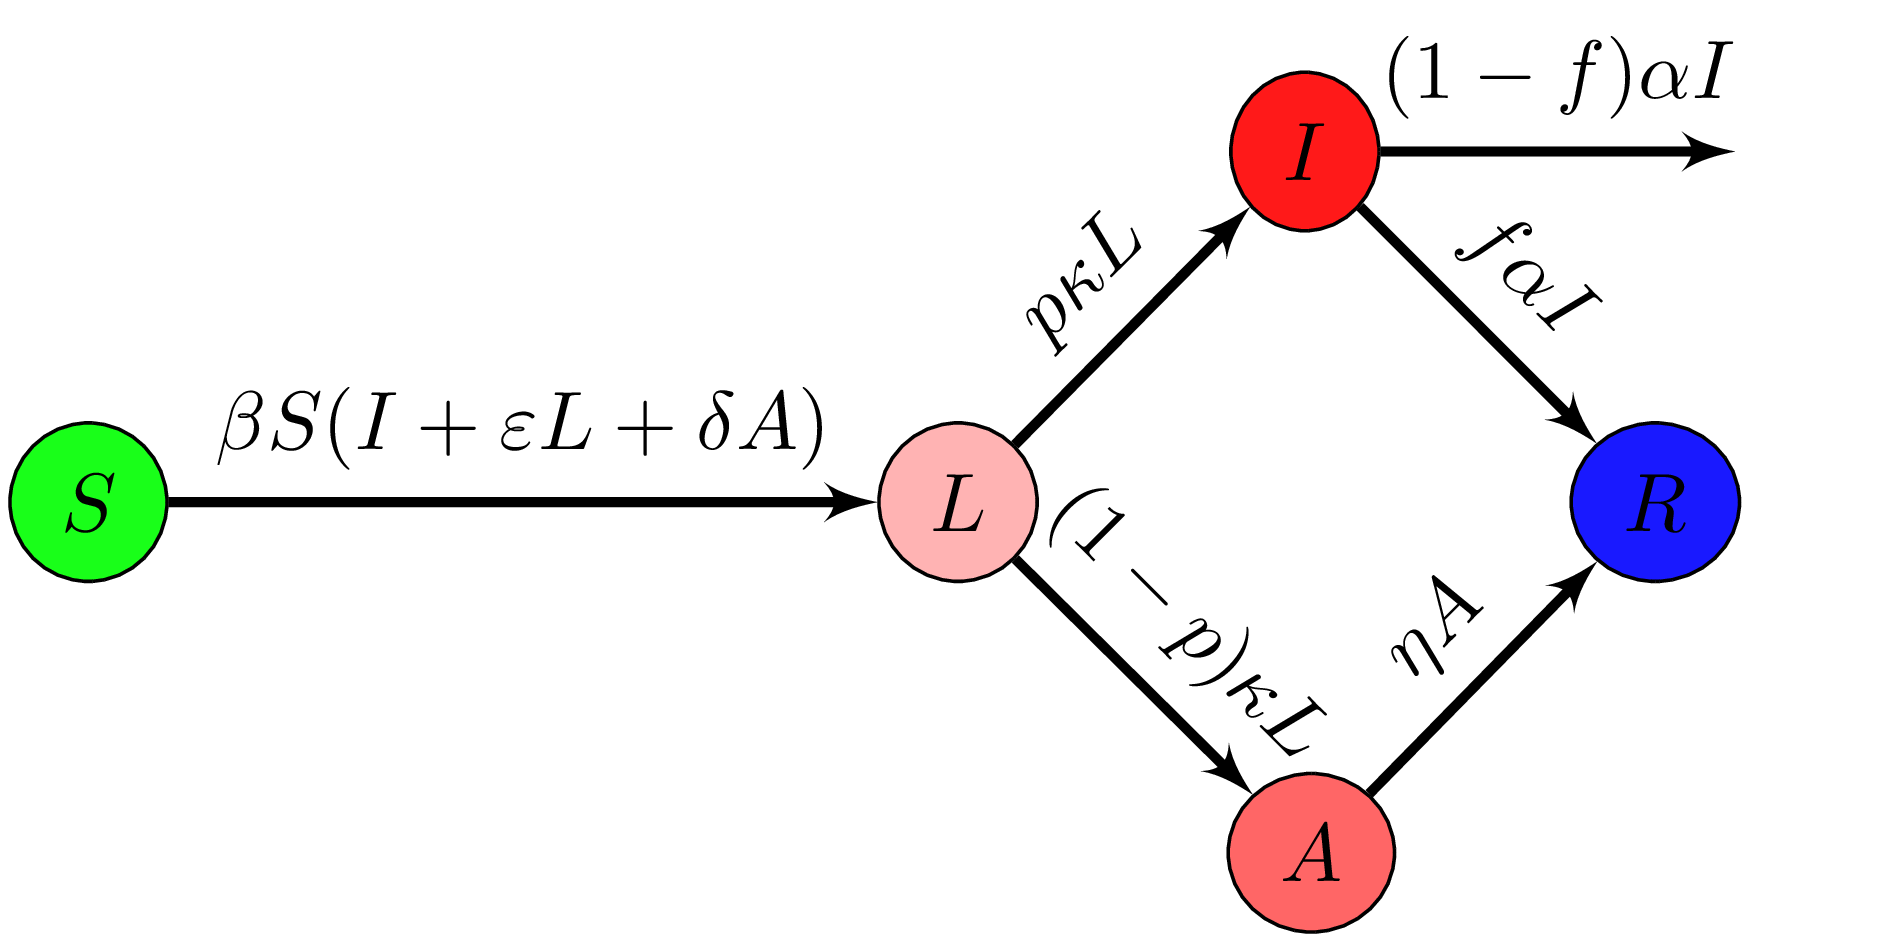
\includegraphics[width=\textwidth]{FIGS/SLIAR_infectiousL}
\end{frame}  


\begin{frame}
Here, $\bS=S$, $\bI=(L,I,A)^T$ and $\bR=R$, so $m=1$, $n=3$ and 
$$
\bh=[\varepsilon\; 1\; \delta],
\quad
\bD=1,
\quad 
\bPi
=\begin{pmatrix}
1 \\ 0 \\0
\end{pmatrix}
\quad\text{and}\quad
\mathbf{V}=
\begin{pmatrix}
\kappa & 0 & 0 \\
-p\kappa & \alpha & 0 \\
-(1-p)\kappa & 0 & \eta
\end{pmatrix}
$$
Incidence is mass action so $\beta(\bE_0)=\beta$ and thus
\begin{align*}
\mathcal{R}_0
&=
\beta\bh\mathbf{V}^{-1}\bPi\bD\bS_0 \\
&=
\beta\;
[\varepsilon\; 1\; \delta]
\begin{pmatrix}
1/\kappa & 0 & 0 \\
p/\alpha & 1/\alpha & 0 \\
(1-p)/\eta & 0 & 1/\eta
\end{pmatrix}
\begin{pmatrix}
1 \\ 0 \\0
\end{pmatrix}
S_0 \\
&=
\beta S_0\left(
\frac{\varepsilon}{\kappa}
+\frac{p}{\alpha}
+\frac{\delta(1-p)}{\eta}
\right)
\end{align*}
\end{frame}  

\begin{frame}
For final size, since $m=1$, we can use $\eqref{eq:final_size_m1}$:
\[
\ln\left(
\frac{S_0}{S_\infty}
\right)
=\frac{\mathcal{R}_0}{S_0}
(S_0-S_\infty)+\beta\bh\mathbf{V}^{-1}\bI_0
\]
\vfill
Suppose $\bI_0=(0,I_0,0)$, then
\[
\ln\left(
\frac{S_0}{S_\infty}
\right)
=\mathcal{R}_0\frac{S_0-S_\infty}{S_0}
+\frac{\beta}{\alpha}I_0
\]
\vfill
If $\bI_0=(L_0,I_0,A_0)$, then
\[
\ln\left(
\frac{S_0}{S_\infty}
\right)
=\mathcal{R}_0\frac{S_0-S_\infty}{S_0}
+\beta\left(
\frac{\varepsilon}{\kappa}
+\frac{p}{\alpha}
+\frac{\delta(1-p)}{\eta}
\right)L_0
+\frac{\beta\delta}{\eta}A_0
+\frac{\beta}{\alpha}I_0
\]
\end{frame}  



%%%%%%%%%%%%%%%%%%%%
%%%%%%%%%%%%%%%%%%%%
\subsection{A model with vaccination}

\begin{frame}{A model with vaccination}
\centering
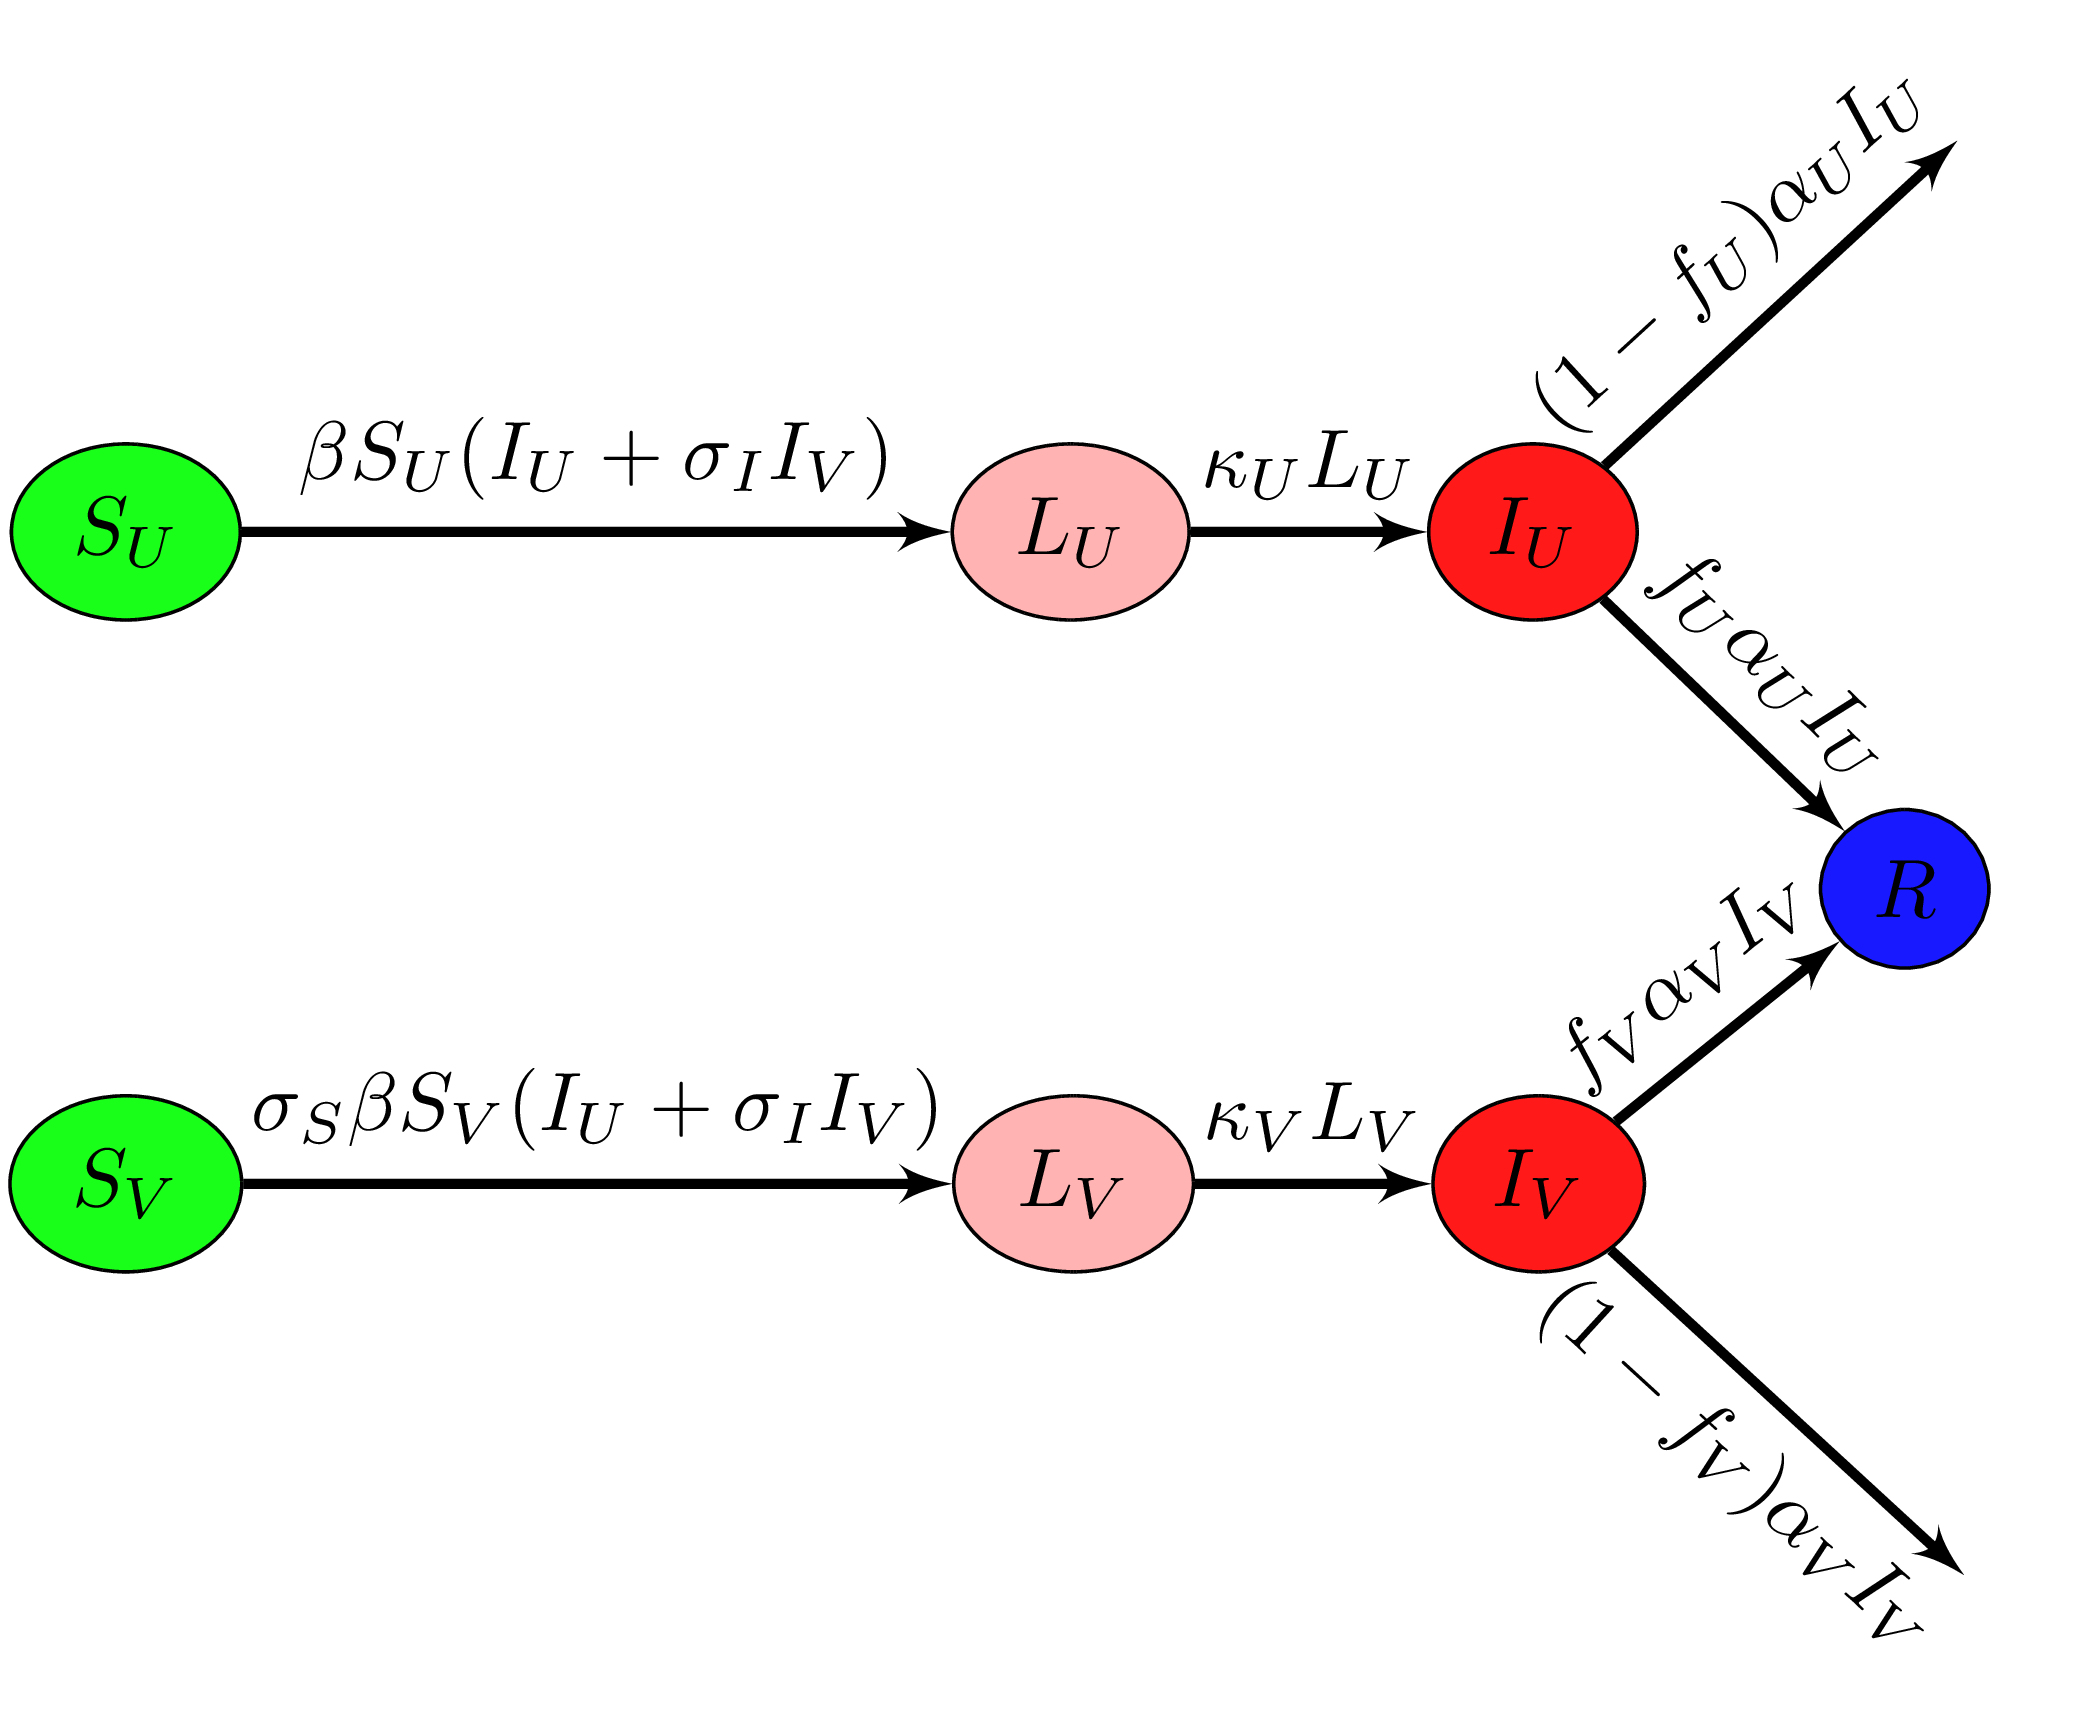
\includegraphics[height=0.95\textheight]{FIGS/SLIR_epidemic_with_vaccination}
\end{frame}  


\begin{frame}{A model with vaccination}
Fraction $\gamma$ of $S_0$ are vaccinated before the epidemic; vaccination reduces probability and duration of infection, infectiousness and reduces mortality
\begin{subequations}
\begin{align}
S_U\pprime &= -\beta S_U[I_U+\sigma_II_V] \\
S_V\pprime &= -\sigma_S\beta S_V[I_U+\sigma_II_V] \\
L_U\pprime &= \beta S_U[I_U+\sigma_II_V]-\kappa_UL_U\\
L_V\pprime &= \sigma_S\beta S_V[I_U+\sigma_II_V]-\kappa_VL_V \\
I_U\pprime &= \kappa_UL_U-\alpha_UI_U \\
I_V\pprime &= \kappa_VL_V-\alpha_VI_V \\
R\pprime &= f_U\alpha_UI_I+f_V\alpha_VI_V
\end{align}
\end{subequations}
with $S_U(0)=(1-\gamma)S_0$ and $S_V(0)=\gamma S_0$
\end{frame}  


\begin{frame}
Here, $m=2$, $n=4$,
\[
\bh = [0\;0\;1\;\sigma_I],\quad
\bD=\begin{pmatrix}
1 & 0 \\ 0 & \sigma_S
\end{pmatrix},\quad
\bPi=
\begin{pmatrix}
1 & 0 \\ 0 & 1 \\ 0 & 0 \\ 0 & 0
\end{pmatrix}
\]
and
\[
\mathbf{V}=
\begin{pmatrix}
\kappa_U & 0 & 0 & 0 \\
0 & \kappa_V & 0 & 0 \\
-\kappa_U & 0 & \alpha_U & 0 \\
0 & -\kappa_V & 0 & \alpha_V
\end{pmatrix}
\]
\end{frame}

\begin{frame}
So
\[
\bGamma=\left[
\frac{\beta}{\alpha_U}\; \frac{\sigma_I\sigma_S\beta}{\alpha_V}
\right],
\quad
\mathcal{R}_c = S_0\beta\left(
\frac{1-\gamma}{\alpha_U}+\frac{\sigma_I\sigma_S\gamma}{\alpha_V}
\right)
\]
and the final size relation is
\begin{multline*}
\ln\left(
\frac{(1-\gamma)S_U(0)}{S_U(\infty)}
\right)
= \\ 
\frac{\beta}{\alpha_U}[(1-\gamma)S_U(0)-S_U(\infty)] \\
+\frac{\sigma_I\beta}{\alpha_V}[\gamma S_V(0)-S_V(\infty)]+\frac{\beta}{\alpha_U}I_0 \\
\end{multline*}
\[
S_V(\infty) = \gamma S_U(0)\left(
\frac{S_U(\infty)}{(1-\gamma)S_0}
\right)^{\sigma_S}
\]
\end{frame}

%%%%%%%%%%%%%%%%%%%%
%%%%%%%%%%%%%%%%%%%%
\subsection{Antiviral resistance}

\begin{frame}{Adapting treatment to counter emergence of resistance}
Arino, Bowman \& Moghadas, \href{https://bmcinfectdis.biomedcentral.com/counter/pdf/10.1186/1471-2334-9-8.pdf}{Antiviral resistance during pandemic influenza: implications for stockpiling and drug use}, \emph{BMC Infectious Disease} (2009)
\vfill
This work was undertaken at the request of the Public Health Agency of Canada during the pandemic preparadness phase prior to the 2009 p-H1N1 pandemic
\vfill
Problem: we have antivirals to use against influenza, either prophylactically or curatively. Using these antivirals may promote the emergence of antiviral-resistant strains. How do we minimise this risk?
\end{frame}


\begin{frame}
\centering
\resizebox{\textwidth}{!}{
  \begin{tikzpicture}[%transform canvas={scale=1.3},
      auto,
      cloud/.style={minimum width={width("N-1")+2pt},
      draw, 
      ellipse,
      fill=gray!20}]
    %% S
    \node [cloud, fill=green!90] at (0,0) (S) {$S$};
    %% Untreated, resistant
    \node [cloud, fill=red!90] at (3,1) (A_r) {$A_r$};
    \node [cloud, fill=red!60] at (3,-1) (I_rU) {$I_{rU}$};
    \node [cloud, fill=blue!60] at (6,0) (R_rU) {$R_{rU}$};
    %% Untreated, sensitive
    \node [cloud, fill=red!90] at (-3,1) (A) {$A$};
    \node [cloud, fill=red!60] at (-3,-1) (I_U) {$I_U$};
    \node [cloud, fill=blue!60] at (-6,0) (R_U) {$R_U$};
    %% Treated
    \node [cloud, fill=red!90] at (-1.5,-3) (I_T) {$I_T$};
    \node [cloud, fill=red!90] at (1.5,-3) (I_rT) {$I_{rT}$};
    \node [cloud, fill=red!90] at (0,-6) (I_Tr) {$I_{Tr}$};
    %% Resistance
    \node [cloud, fill=blue!60] at (-4.5,-3) (R_T) {$R_T$};
    \node [cloud, fill=blue!60] at (4.5,-3) (R_rT) {$R_{rT}$};
    \node [cloud, fill=blue!60] at (3,-6) (R_Tr) {$R_{Tr}$};
    %%
    %% Infections
    \path [line, very thick] (S) to node [midway,above,sloped] (TextNode) {$(1-p)fS$} (A);
    \path [line, very thick] (S) to node [midway,below,sloped] (TextNode) {$(1-q)pfS$} (I_U);
    \path [line, very thick] (S) to node [midway,above,sloped] (TextNode) {$(1-p)gS$} (A_r);
    \path [line, very thick] (S) to node [midway,below,sloped] (TextNode) {$(1-q)pgS$} (I_rU);
    \path [line, very thick] (S) to node [near end,above,sloped] (TextNode) {$qpfS$} (I_T);
    \path [line, very thick] (S) to node [midway,below,sloped] (TextNode) {$qpgS$} (I_rT);
    %% Removals
    \path [line, very thick] (A) to node [midway,below,sloped] (TextNode) {$\mu_AA$} (R_U);
    \path [line, very thick] (I_U) to node [midway,below,sloped] (TextNode) {$(d_U+\mu_U)I_U$} (R_U);
    \path [line, very thick] (A_r) to node [midway,below,sloped] (TextNode) {$\mu_AA_r$} (R_rU);
    \path [line, very thick] (I_rU) to node [midway,below,sloped] (TextNode) {$(d_{rU}+\mu_U)I_{rU}$} (R_rU);
    \path [line, very thick] (I_T) to node [midway,below,sloped] (TextNode) {$(d_T+\mu_T)I_T$} (R_T);
    \path [line, very thick] (I_rT) to node [midway,below,sloped] (TextNode) {$(d_{rU}+\mu_U)I_{rT}$} (R_rT);
    \path [line, very thick] (I_Tr) to node [midway,below,sloped] (TextNode) {$(d_{Ur}+\mu_U)I_{Tr}$} (R_Tr);
    %% I_T transitions
        \path [line, very thick] (I_T) to node [midway,below,sloped] (TextNode) {$\alpha I_T$} (I_Tr);
    \path [line, very thick] (I_Tr) to node [midway,below,sloped] (TextNode) {$\gamma I_{Tr}$} (I_rT);
  \end{tikzpicture}
}
\end{frame}

\begin{frame}
\centering
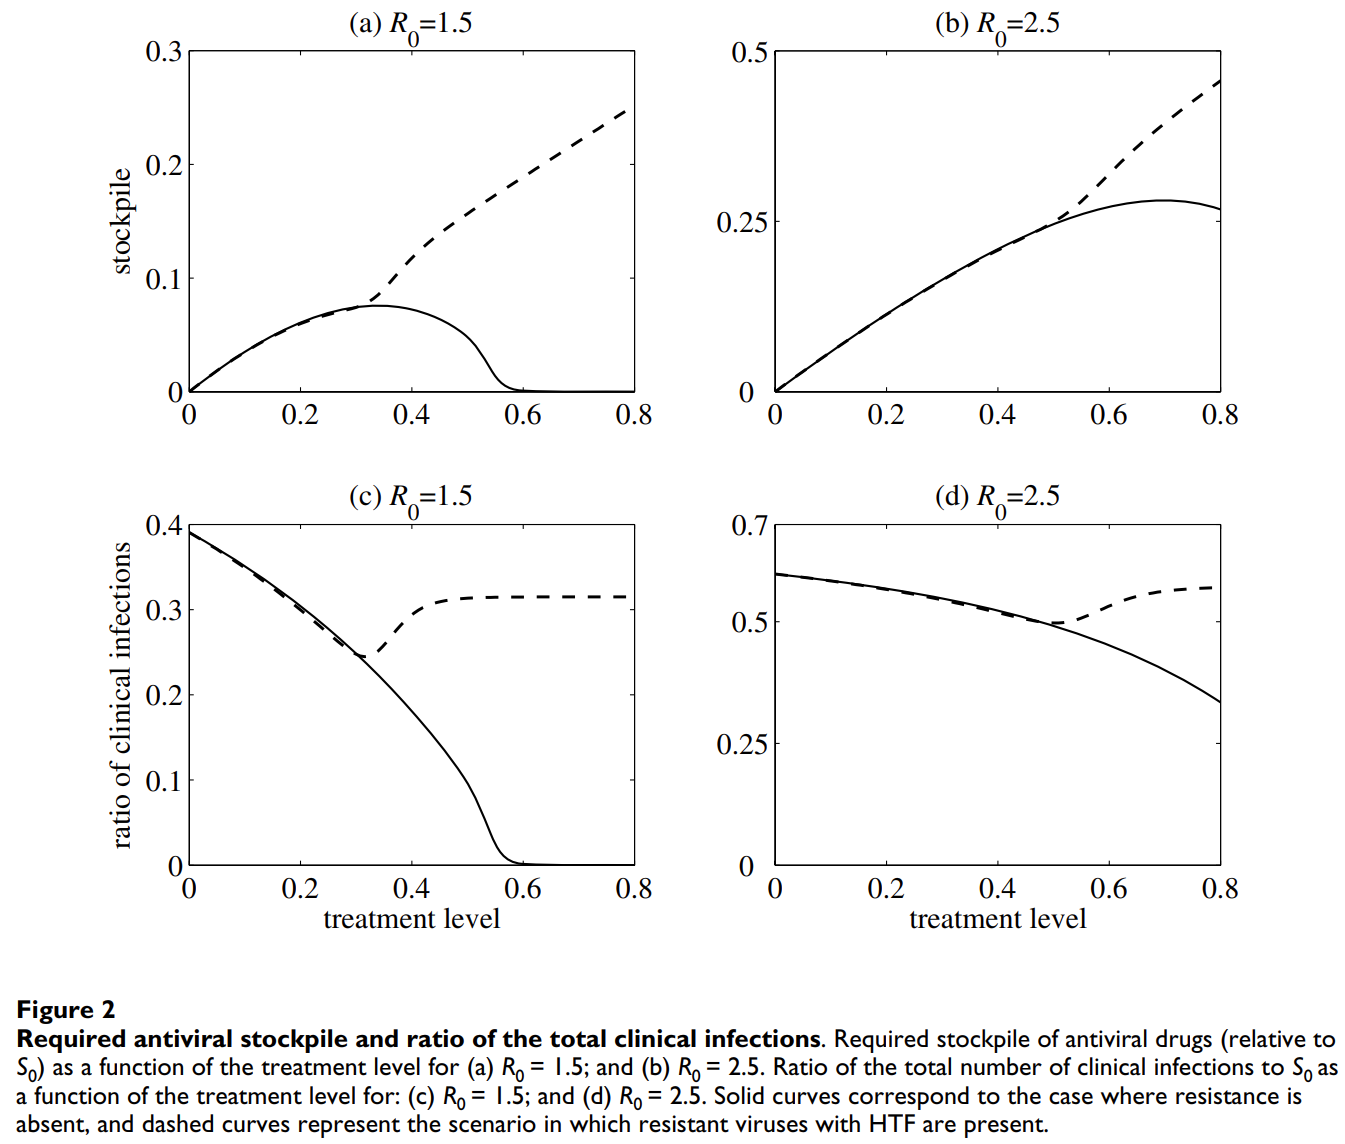
\includegraphics[height=\textheight]{FIGS/ABM-role-of-resistance}
\end{frame}

\begin{frame}
\centering
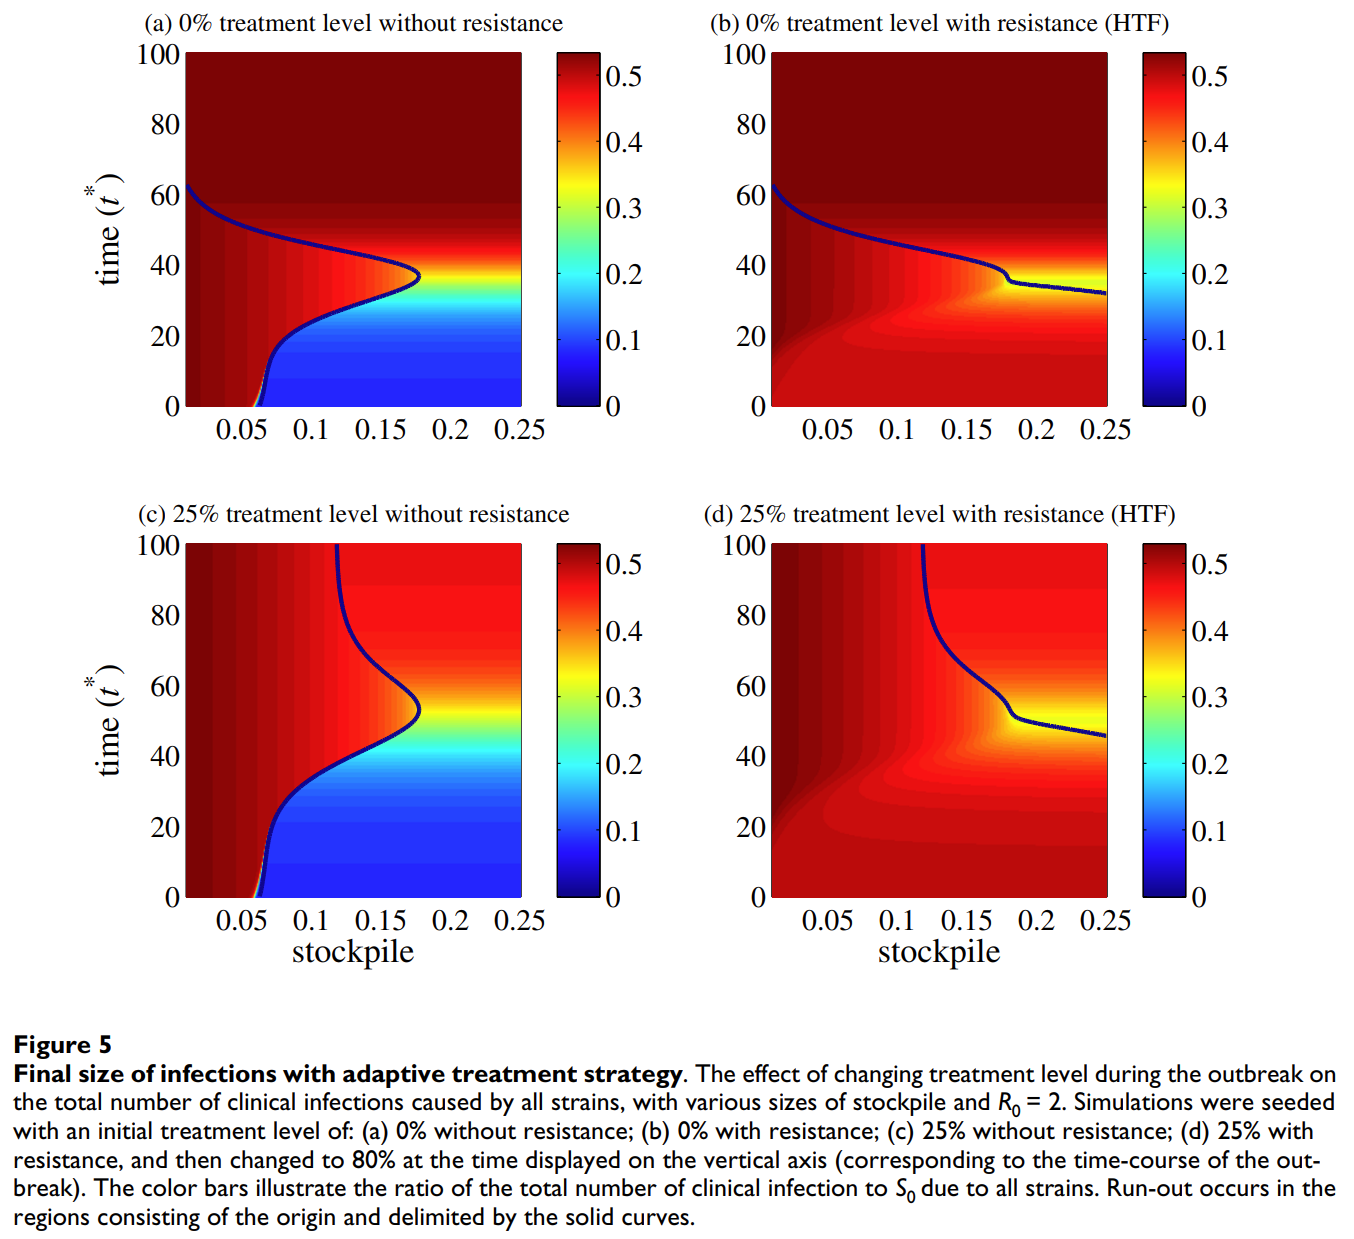
\includegraphics[height=\textheight]{FIGS/ABM-heatmaps}
\end{frame}

%%%%%%%%%%%%%%%%%%%
%%%%%%%%%%%%%%%%%%%
\subsection{A COVID-19 model}

\begin{frame}
Arino \& Portet, \href{http://dx.doi.org/10.1016/j.idm.2020.04.002}{A simple model for COVID-19}, \emph{Infectious Disease Modelling} (2020)
\vfill
Extends the SLIAR model to take into account non-exponentially distributed stage durations (see lecture on Stochastic systems)
\end{frame}

\begin{frame}{The original model (well, almost the first one)}
\centering
\def\horzskip{*2}
\def\vertskip{*2}
\begin{tikzpicture}[auto, %node distance = 2cm, auto,
	cloud/.style={minimum width={width("N-1")+2pt},
		draw, ellipse,fill=red!20}]
	\node [cloud] (S) at (0,0) {$S$};
	\node [cloud] (L1) at (1\horzskip,0) {$L_1$};
	\node [cloud] (L2) at (2\horzskip,0) {$L_2$};
	\node [cloud,fill=blue!20] (I1) at (3\horzskip,-1\vertskip) {$I_1$};
	\node [cloud] (A1) at (3\horzskip,1\vertskip) {$A_1$};
	\node [cloud,fill=blue!20] (I2) at (4\horzskip,-1\vertskip) {$I_2$};
	\node [cloud] (A2) at (4\horzskip,1\vertskip) {$A_2$};
	\node [cloud,fill=blue!20] (RI) at (5\horzskip,0) {$R_I$};
	\node [cloud] (RA) at (5\horzskip,1\vertskip) {$R_A$};
	\node [cloud,, fill=blue!20] (D) at (5\horzskip,-2\vertskip) {$D$};
	%% Infections
	\path [line, very thick] (S) to node [midway,above] (TextNode) {$\Phi S$} (L1);
	\path [line, very thick] (L1) to node [midway,above] (TextNode) {$\varepsilon L_1$} (L2);
	\path [line, very thick] (L2) to node [midway,below,sloped] (TextNode) {$(1-\pi)\varepsilon L_2$} (I1);
	\path [line, very thick] (L2) to node [midway,below,sloped] (TextNode) {$\pi\varepsilon L_2$} (A1);
	\path [line, very thick] (I1) to node [midway, above] (TextNode) {$\gamma I_1$} (I2);
	\path [line, very thick] (A1) to node [midway, above] (TextNode) {$\gamma A_1$} (A2);
	\path [line, very thick] (I2) to node [midway,above,sloped] (TextNode) {$(1-\delta)\gamma I_2$} (RI);
	\path [line, very thick] (A2) to node [midway, above] (TextNode) {$\gamma A_2$} (RA);
	\path [line, very thick] (I2) to node [midway,below,sloped] (TextNode) {$\delta\gamma I_2$} (D);
\end{tikzpicture}
\end{frame}


\begin{frame}{Reinterpreting terms}
Here $D$ stands for \emph{detected}, $U$ is \emph{undetected}
\vfill
\centering
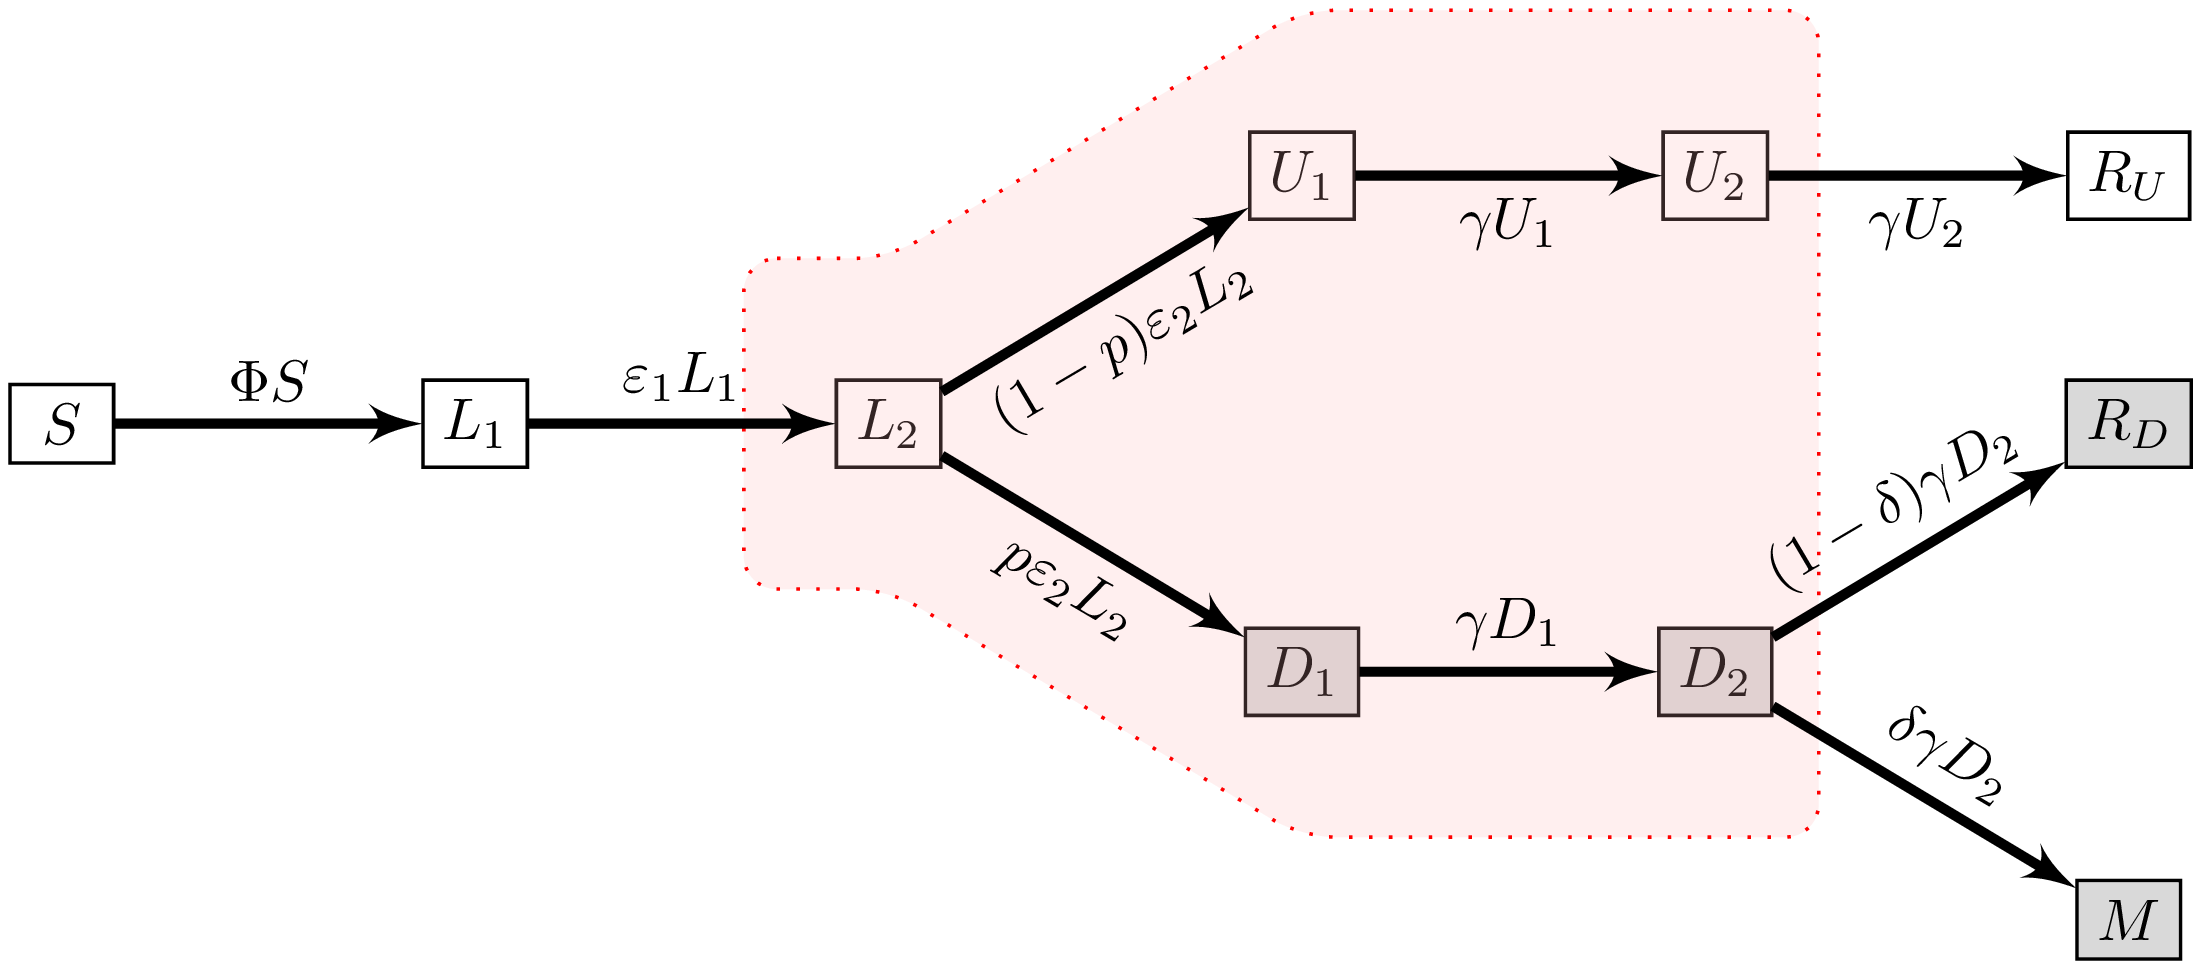
\includegraphics[width=\textwidth]{FIGS/figure_SLDURM_base_model_with_different_epsilon_and_infectious_compartments}
\end{frame}

\begin{frame}{Working out when the first COVID-19 case occurred}
\bbullet Details of emergence and precise timeline before amplification started unknown
\vfill
\bbullet Amplification in Wuhan
\begin{itemize}
\item Cluster of pneumonia cases mostly related to the Huanan Seafood Market
\item 27 December 2019: first report to local government
\item 31 December 2019: publication
\item 8 January 2020: identification of SARS-CoV-2 as causative agent
\item $\sim$ 23 January 2020: lockdown Wuhan and Hubei province + face mask mandates
\end{itemize}
\vfill
\bbullet By 2020-01-29, virus in all provinces of mainland CHN
\end{frame}


\begin{frame}{Evidence of earlier spread}
\bbullet Report to Wuhan authorities on 27 December 2019
\vfill
\bbullet First export detections in Thailand and Japan on 13 and 16 January 2020 (with actual importations on 8 and 6 January)
\vfill
$\implies$ amplification must have been occuring for a while longer
\vfill
\bbullet France: sample taken from 42-year-old male (last foreign travel to Algeria in August 2019) who presented to ICU on 27 December 2019
\vfill
\bbullet Retrospective studies in United Kingdom and Italy also showed undetected COVID-19 cases in prepandemic period
\end{frame}

\begin{frame}{Untangling the first case issue}
\bbullet Robert, Rossman \& Jaric. Dating first cases of COVID-19. \emph{PLoS Pathogens} (2021)

Find likely timing of first case of COVID-19 in China as November 17 (95\% CI October 4)
\vfill
\bbullet Pekar, Worobey, Moshiri, Scheffler \& Wertheim. Timing the SARS-CoV-2 index case in Hubei province. \emph{Science} (2021)

Period between mid-October and mid-November 2019 is plausible interval when the first case of SARS-CoV-2 emerged in Hubei province
\vfill
Important when trying to understand global spread, so let me illustrate with the model I used, taking into account model evolution since
\end{frame}

\begin{frame}{Back-calculating the start of spread (example of China)}
Cumulative confirmed case counts in China as reported to WHO was $c=547$ cases on $t_c=\textrm{2020-01-22}$
\vfill
Let $u$ be a point in parameter space. Solve ODE numerically over $[0,t]$, with $S(0)$ the population of China, $L_1(0)=1$ and other state variables 0. This gives a solution $x(t,t_0=0,u)$
\vfill
Extracting $L_2(t,t_0=0,u)$ from this solution, obtain cumulative number of new detections as
\[
C(t) = \int_{t_0=0}^{t} p\varepsilon_2 L_2(s,t_0,u)\ ds
\]
\vfill
Let $t^\star$ be s.t. $C(t^\star)=547$; then $t_i=\textrm{2020-01-22}-t^\star$
\end{frame}

\begin{frame}
\centering
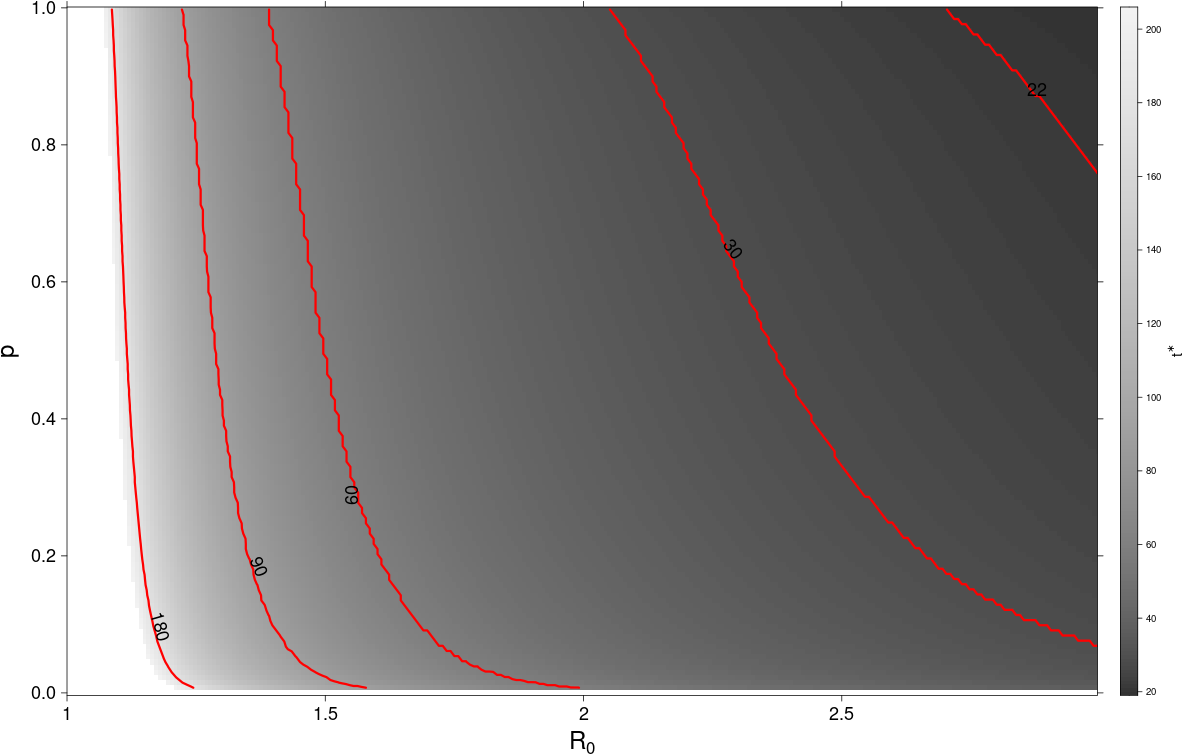
\includegraphics[width=\textwidth]{FIGS/start_time_vs_R0_and_p.png}
\end{frame}

%%%%%%%%%%%%%%%%%%%
%%%%%%%%%%%%%%%%%%%
%%%%%%%%%%%%%%%%%%%
%%%%%%%%%%%%%%%%%%%
\section{The SLIRS models and friends}

%%%%%%%%%%%%%%%%%%%
%%%%%%%%%%%%%%%%%%%
\subsection{SIS models}


\begin{frame}{Note on demography}
\bbullet We have already discussed some different possible forms for demography
\vfill
\bbullet In the models with demography here, unless otherwise required, we use demography such that for the total population
\[
N\pprime = b - dN
\]
\end{frame}


\begin{frame}{Simplifying the SIRS model}
\begin{minipage}{0.2\textwidth}
  \def\skip{*-1.5}
  \begin{tikzpicture}[scale=1, transform shape]
    %% Regular nodes
    \node [circle, fill=green!50, text=black] at (0,0) (S) {$S$};
    \node [circle, fill=red!90, text=black] at (0,1\skip) (I) {$I$};
    %% Fake nodes for arrows
    \node [above=0.75cm of S] (birth) {};
    \node [left=0.5cm of S] (dS) {};
    \node [left=0.5cm of I] (dI) {};
    %% Flows
    \path [line, very thick] (birth) to node [midway, left] (TextNode) {$b$} (S);
    \path [line, very thick] (S) to node [midway, above] (TextNode) {$dS$} (dS);
    \path [line, very thick] (I) to node [midway, below] (TextNode) {$dI$} (dI);
    \path [line, very thick, bend right] (S) to node [midway, left] (TextNode) {$\beta SI$} (I);
    \path [line, very thick, bend right] (I) to node [midway, right] (TextNode) {$\gamma I$} (S);
  \end{tikzpicture}    
\end{minipage}
\begin{minipage}{0.75\textwidth}
\bbullet We have already seen the epidemic KMK SIR model and the endemic SIRS model
\vskip0.5cm
\bbullet By making some simplifications of the endemic SIRS model, we obtain the SIS model: assume the time spent in the $R$ compartment goes to zero, i.e., $\nu\to\infty$
\end{minipage}
\vfill
The main characteristics of the model are the same as the SIRS
\end{frame}

\begin{frame}
\begin{minipage}{0.2\textwidth}
  \def\skip{*-1.5}
  \begin{tikzpicture}[scale=1, transform shape]
    %% Regular nodes
    \node [circle, fill=green!50, text=black] at (0,0) (S) {$S$};
    \node [circle, fill=red!90, text=black] at (0,1\skip) (I) {$I$};
    %% Fake nodes for arrows
    \node [above=0.75cm of S] (birth) {};
    \node [left=0.5cm of S] (dS) {};
    \node [left=0.5cm of I] (dI) {};
    %% Flows
    \path [line, very thick] (birth) to node [midway, left] (TextNode) {$b$} (S);
    \path [line, very thick] (S) to node [midway, above] (TextNode) {$dS$} (dS);
    \path [line, very thick] (I) to node [midway, below] (TextNode) {$dI$} (dI);
    \path [line, very thick, bend right] (S) to node [midway, left] (TextNode) {$\beta SI$} (I);
    \path [line, very thick, bend right] (I) to node [midway, right] (TextNode) {$\gamma I$} (S);
  \end{tikzpicture}    
\end{minipage}
\begin{minipage}{0.75\textwidth}
\begin{subequations}\label{sys:SIS}
\begin{align}
S\pprime &= b +\gamma I -dS - \beta SI \label{sys:SIS_dS} \\
I\pprime &= \beta SI -(d+\gamma) I
\end{align}
\end{subequations}
with initial conditions $S(0)=S_0\geq 0$ and $I(0)=I_0\geq 0$
\end{minipage}
\vfill
Clearly, the DFE is similar as for the SIRS
\[
\bE_0:=(S^\star,I^\star)=(N^\star,0)
\]
with $N^\star = b/d$. Also easy to check (exercise!) that
\[
\R_0 = \frac{\beta}{d+\gamma}
\]
\end{frame}

%%%%%%%%%%%%%%
%%%%%%%%%%%%%%
\subsection{SLIRS model with constant population}

\frame{\frametitle{Incubation periods}
\begin{itemize}
\item SIS and SIR: progression from S to I is instantaneous
\vfill
\item Several incubation periods:
\end{itemize}
\begin{center}
\begin{tabular}{l|l}
Disease & Incubation period \\
\hline
Yersinia Pestis & 2-6 days \\
Ebola haemorrhagic fever (HF) & 2-21 days \\
Marburg HF & 5-10 days \\
Lassa fever & 1-3 weeks \\
Tse-tse & weeks--months \\
HIV/AIDS & months--years
\end{tabular}
\end{center}
}

\frame{\frametitle{Hypotheses}
\begin{itemize}
\item There is demography
\item New individuals are born at a constant rate $b$
\item
There is no vertical transmssion: all ``newborns'' are susceptible
\item The disease is non lethal, it causes no additional mortality
\item New infections occur at the rate $f(S,I,N)$
\item There is a period of incubation for the disease
\item There is a period of time after recovery during which the disease confers immunity to reinfection (immune period)
\end{itemize} 
}

\frame{\frametitle{SLIRS}
\begin{minipage}{0.2\textwidth}
  \def\skip{*-1.5}
  \begin{tikzpicture}[scale=1, transform shape]
    %% Regular nodes
    \node [circle, fill=green!50, text=black] at (0,0) (S) {$S$};
    \node [circle, fill=red!50, text=black] at (0,1\skip) (L) {$L$};
    \node [circle, fill=red!90, text=black] at (0,2\skip) (I) {$I$};
    \node [circle, fill=blue!50, text=black] at (0,3\skip) (R) {$R$};
    %% Fake nodes for arrows
    \node [above=0.75cm of S] (birth) {};
    \node [left=0.5cm of S] (dS) {};
    \node [left=0.5cm of L] (dL) {};
    \node [left=0.5cm of I] (dI) {};
    \node [left=0.5cm of R] (dR) {};
    %% Flows (demography)
    \path [line, very thick] (birth) to node [midway, left] (TextNode) {$b$} (S);
    \path [line, very thick] (S) to node [midway, above] (TextNode) {$dS$} (dS);
    \path [line, very thick] (L) to node [midway, below] (TextNode) {$dL$} (dL);
    \path [line, very thick] (I) to node [midway, below] (TextNode) {$dI$} (dI);
    \path [line, very thick] (R) to node [midway, below] (TextNode) {$dR$} (dR);
    %% Flows (demography)
    \path [line, very thick] (S) to node [midway, left] (TextNode) {$f(S,I,N)$} (L);
    \path [line, very thick] (L) to node [midway, left] (TextNode) {$\varepsilon L$} (I);
    \path [line, very thick] (I) to node [midway, left] (TextNode) {$\gamma I$} (R);
    \draw [>=latex,->, thick, rounded corners] (R) -- (0.75,3\skip) -- (0.75,0) node[midway,above,sloped] {$\nu R$} -- (S);
  \end{tikzpicture}    
\end{minipage}
\quad
\begin{minipage}{0.7\textwidth}
The model is as follows:
\begin{subequations}\label{sys:SLIRS}
\begin{align}
S\pprime &= b+\nu R-dS-f(S,I,N) \label{sys:SLIRS_dS} \\
L\pprime &= f(S,I,N) -(d+\varepsilon)L \label{sys:SLIRS_dL} \\
I\pprime &= \varepsilon L -(d+\gamma)I \label{sys:SLIRS_dI} \\
R\pprime &= \gamma I-(d+\nu)R \label{sys:SLIRS_dR} 
\end{align}
\end{subequations}
\vfill
Meaning of the parameters:
\begin{itemize}
\item $1/\varepsilon$ average duration of the incubation period
\item $1/\gamma$ average duration of infectious period
\item $1/\nu$ average duration of immune period
\end{itemize}
\end{minipage}
}



%%%%%%%%%%%%%%%%%%%%%%%
%%%%%%%%%%%%%%%%%%%%%%%
\subsection{Computing $\R_0$ more efficiently}


\frame{\frametitle{The basic reproduction number $\R_0$}
Used frequently in epidemiology (not only math epi)
\begin{definition}[$R_0$]
The basic reproduction number $\R_0$ is the average number of secondary cases generated by the introduction of an infectious individual in a wholly susceptible population
\end{definition}
\begin{itemize}
\item If $\R_0<1$, then on average, each infectious individual infects less than one other person, so the epidemic has chances of dying out
\item If $\R_0>1$, then on average, each infectious individual infects more than one other person and the disease can become established in the population (or there will be a major epidemic)
\end{itemize}
}

\frame{\frametitle{Computation of $\R_0$}
Mathematically, $\R_0$ is a bifurcation parameter aggregating some of the model parameters and such that the disease free equilibrium (DFE) loses its local asymptotic stability when $\R_0=1$ is crossed from left to right
\vfill
\begin{itemize}
\item
As a consequence, $\R_0$ is found by considering the spectrum of the Jacobian matrix of the system evaluated at the DFE
\vfill
\item
The matrix quickly becomes hard to deal with (size and absence of ``pattern'') and the form obtained is not unique, which is annoying when trying to interpret $\R_0$
\end{itemize}
}

\frame{\frametitle{The next generation operator}
Diekmann and Heesterbeek, characterized in the ODE context by van den Driessche and Watmough
\vfill
Consider only individuals harbouring the pathogen, in a vector $\I$, and form the vectors
\begin{itemize}
\item
$\F$ of infection fluxes
\item
$\V$ of other fluxes (with $-$ sign)
\end{itemize}
so that
\[
\I\pprime=\F-\V
\]
\vfill
Then compute the Fr\'echet derivatives $D\F$ and $D\V$ with respect to the infected variables $\I$ and evaluate $F=D\F(DFE)$ and $V=D\V(DFE)$. Then
\[
\R_0=\rho(FV^{-1})
\]
where $\rho$ is the spectral radius
}

\frame{\frametitle{Short summary of van den Driessche and Watmough}
\begin{theorem}[van den Driessche and Watmough]\label{th:R0_VdDW}
Suppose that the DFE exists. Let then $\R_0$ be defined by
\[
\R_0=\rho(FV^{-1})
\]
with matrices $F$ and $V$ as indicated before. Then,
\begin{itemize}
\item if $\R_0<1$, the DFE is LAS,
\item if $\R_0>1$, the DFE is unstable.
\end{itemize}
\end{theorem}
}

\frame{\frametitle{Example of the SLIRS model \eqref{sys:SLIRS}}
Variation of the infected variables in \eqref{sys:SLIRS} are described by
\begin{align*}
L\pprime &= f(S,I,N)-(\varepsilon+d) L \\
I\pprime &= \varepsilon L -(d+\gamma) I
\end{align*}
Write
\begin{equation}
\I\pprime = 
\left(
\begin{matrix}
L \\
I
\end{matrix}
\right)'
=\left(
\begin{matrix}
f(S,I,N) \\
0
\end{matrix}
\right)
-
\left(
\begin{matrix}
(\varepsilon+d) L \\
(d+\gamma) I-\varepsilon L
\end{matrix}
\right)=:\mathcal{F}-\mathcal{V}
\end{equation}
}


\frame{
Denote
\[
f_L^{\,\star}:=
\left.\frac{\partial}{\partial L}f
\right|_{(S,I,R)=\bE_0}
\quad\quad 
f_I^{\,\star}:=
\left.\frac{\partial}{\partial I}f
\right|_{(S,I,R)=\bE_0}
\]
the values of the partials of the incidence function at the DFE $\bE_0$
\vfill
Compute the Jacobian matrices of vectors $\F$ and $\V$ at the DFE $\bE_0$
\begin{equation}
F=\left(
\begin{matrix}
f_L^{\,\star} & f_I^{\,\star} \\
0 & 0
\end{matrix}
\right)
\quad\text{and}\quad
V=\left(
\begin{matrix}
\varepsilon+d & 0 \\
-\varepsilon & d+\gamma
\end{matrix}
\right)
\end{equation}
}

\frame{
Thus
\[
V^{-1}=\frac{1}{(d+\varepsilon)(d+\gamma)}
\left(
\begin{matrix}
d+\gamma & 0 \\
\varepsilon & d+\varepsilon
\end{matrix}
\right)
\]
\vfill
Also, in the case $N$ is constant, $\partial f/\partial L=0$ and thus
\[
FV^{-1}=\frac{f_I^{\,\star}}
{(d+\varepsilon)(d+\gamma)}
\left(
\begin{matrix}
\varepsilon 
& d+\varepsilon  \\
0 & 0
\end{matrix}
\right)
\]
\vfill
As a consequence,
\[
\R_0=\varepsilon
\frac{f_I^{\,\star}}
{(d+\varepsilon)(d+\gamma)}
\]
}


\frame{
\begin{theorem}\label{th:R0_SEIRS}
Let
\begin{equation}\label{eq:R0_SEIRS}
\R_0=
\frac{\varepsilon f_I^{\,\star}}
{(d+\varepsilon)(d+\gamma)}
\end{equation}
Then
\begin{itemize}
\item if $\R_0<1$, the DFE is LAS
\item if $\R_0>1$, the DFE is unstable
\end{itemize}
\end{theorem}
\vfill
It is important here to stress that the result we obtain concerns the \textbf{local} asymptotic stability. We see later that even when $\R_0<1$, there can be several locally asymptotically stable equilibria
}


\frame{\frametitle{Application}
The DFE is
\[
(\bar S,\bar L,\bar I,\bar R)=(N,0,0,0)
\]
\begin{itemize}
\item Mass action incidence (frequency-dependent contacts):
 \[
f_I^{\,\star}=\beta\bar S \Rightarrow\R_0 =
\frac{\epsilon\beta N}{(\epsilon+d)(\gamma+d)} 
\]
\item Standard incidence (proportion-dependent contacts):
\[
f_I^{\,\star}=\frac{\beta\bar S}{N}
\Rightarrow\R_0 = \frac{\epsilon\beta}{(\epsilon+d)(\gamma+d)}
\]
\end{itemize}
}


\frame{\frametitle{Links between SLIRS-type models}
{ %\footnotesize
\begin{align*}
S\pprime&=b+\nu R-dS-f(S,I,N) \\
L\pprime&=f(S,I,N)-(d+\varepsilon) L \\
I\pprime&=\varepsilon L-(d+\gamma)I \\
R\pprime&=\gamma I-(d+\nu)R
\end{align*}}
\begin{center}
\begin{tabular}{c|l}
\hline
SLIR & SLIRS where $\nu=0$ \\
SLIS & Limit of SLIRS when $\nu\to\infty$ \\
SLI & SLIR where $\gamma=0$ \\
SIRS & Limit of SLIRS when $\varepsilon\to\infty$ \\
SIR & SIRS where $\nu=0$ \\
SIS & Limit of SIRS when $\nu\to\infty$ \\
& Limit SLIS when $\varepsilon\to\infty$ \\
SI & SIS where $\nu=0$ 
\end{tabular}
\end{center}
}

\frame{\frametitle{Values of $\R_0$}
$(\bar S,\bar I,\bar N)$ values of $S,I$ and $N$ at DFE. Denote $\bar f_I=\partial f/\partial I(\bar S,\bar I,\bar N)$.
\begin{center}
\begin{tabular}{c|c}
\hline
SLIRS & 
$\frac{\varepsilon\bar f_I}{(d+\varepsilon)(d+\gamma)}$ \\
SLIR & 
$\frac{\varepsilon\bar f_I}{(d+\varepsilon)(d+\gamma)}$ \\
SLIS & 
$\frac{\varepsilon\bar f_I}{(d+\varepsilon)(d+\gamma)}$ \\
SLI & 
$\frac{\varepsilon\bar f_I}{(d+\varepsilon)(d+\gamma)}$ \\
& \\
SIRS & 
$\frac{\varepsilon\bar f_I}{d+\gamma}$ \\
SIR & $\frac{\bar f_I}{d+\gamma}$ \\
SIS & $\frac{\bar f_I}{d+\gamma}$ \\
SI & $ \frac{\bar f_I}{d+\gamma}$ 
\end{tabular}
\end{center}
}


%%%%%%%%%%%%%%%%
%%%%%%%%%%%%%%%%
\subsection{Global properties of the SLIRS model}

\frame{\frametitle{Lyapunov function for SLIR and SLIS}
(A. Korobeinikov) Consider an SLIR in constant population (normed to 1), with vertical transmission.
\begin{subequations}\label{sys:SEIR_vert_transmission}
\begin{align}
S\pprime &= d-\beta SI -pdI-qdL-dS \\
L\pprime &= \beta SI +pdI-(\varepsilon+d-qd)L \\
I\pprime &= \varepsilon L-(\gamma+d)I
\end{align}
\end{subequations}
\vfill
$p$ proportion of progeny of $I$ that are $I$ at birth, $q$ proportion of progeny of $L$ that are $L$ at birth.
\vfill
$R$ does not play a role in the dynamics of \eqref{sys:SEIR_vert_transmission}, it is not shown.
}

\frame{\frametitle{Equilibria}
\begin{itemize}
\item DFE: $\bE_0=(1,0,0)$.
\item EEP: $\bE_\star=(S^\star,L^\star,I^\star)$ with
{\footnotesize
\[
S^\star=\frac 1{\R_0^v}\quad L^\star=\frac{d}{\varepsilon+d}\left(1-\frac
  1{\R_0^v}\right) 
\quad
I^*=\frac{d\varepsilon}{(\varepsilon+d)(\gamma+d)}\left(1-\frac
  1{\R_0^v}\right) 
\]}
\end{itemize}
where 
\[
\R_0^v=\frac{\beta\varepsilon}
{(\gamma+d)(\varepsilon+d)-qd(\varepsilon+d)-pd\varepsilon}
\]
is the basic reproduction number with vertical transmission
\vfill
We have $\R_0=\R_0^v$ $\iff$ $p=q=0$ or $\R_0^v=\R_0=1$
\vfill
$\bE_\star$ exists (in a biologically plausible way) only when $\R_0^v>1$
}


\frame{
Consider the Goh Lyapunov function
\[
V=\sum a_i(x_i-x_i^\star \ln x_i)
\]
\vfill
\begin{theorem}
\begin{itemize}
\item If $\R_0>1$, then \eqref{sys:SEIR_vert_transmission} has the globally asymptotically stable equilibrium $\bE_\star$
\item If $\R_0\leq 1$, then \eqref{sys:SEIR_vert_transmission} has the globally asymptotically stable equilibrium $\bE_0$, $\bE_\star$ is not biologically plausible
\end{itemize}
\end{theorem}
}

\begin{frame}{Li, Muldowney and van den Driessche} 
Study an SLIRS model with incidence of the form
\begin{equation}\label{eq:g_incidence}
f(S,I,N)=\beta g(I)S
\end{equation}
where $g$ is such that $g(0)=0$, $g(I)>0$ for $I\in(0,1]$ and $g\in
C^1(0,1]$
\vfill
They normalise the total population, so that $S+L+I+R=1$
\vfill
They make the following asumption about $g$:
\begin{description}
\item[(H)]$c=\lim_{I\to 0^+} \frac{g(I)}{I}\leq +\infty$; when
$0<c<+\infty$, $g(I)\leq cI$ for all sufficiently small $I$
\end{description}
\end{frame}

\frame{
We have 
\[
\frac{\partial\bar f}{\partial I}=\beta\frac{\partial\bar g}{\partial I}
\]
\vfill
Since $\dfrac{\partial\bar g}{\partial I}=\lim_{I\to 0^+}
\dfrac{g(I)}{I}=c$,
\[
\R_0=\frac{c\beta\varepsilon}
{(d+\varepsilon)(d+\gamma)}
\]
\vfill
The LAS results already established hold here, since \eqref{eq:g_incidence} is a special case of the function $f$ with which the results were obtained
}


\frame{
The system is \defword{uniformly persistent} if there exists $0<\varepsilon_0<1$ s.t. any solution $(S(t),L(t),I(t),R(t))$ of \eqref{sys:SLIRS} with initial condition $(S(0),L(0),I(0),R(0))\in
\overset{\circ}{\Gamma}$ satisfies
\begin{equation}\label{eq:SEIRS_persist}
\begin{array}{c}
\liminf_{t\to\infty} S(t)\geq \varepsilon_0,\quad 
\liminf_{t\to\infty} E(t)\geq \varepsilon_0 \\
\liminf_{t\to\infty} I(t)\geq \varepsilon_0,\quad 
\liminf_{t\to\infty} R(t)\geq \varepsilon_0
\end{array}
\end{equation}
\vfill
\begin{theorem}\label{th:persist_SEIRS}
If $g(I)$ satisfies hypothesis (\textbf{H}), then \eqref{sys:SLIRS} with incidence \eqref{eq:g_incidence} is uniformly persistent iff $\R_0>1$
\end{theorem}
}


\frame{
\begin{theorem}\label{th:gas_SEIRS}
Suppose that incidence \eqref{eq:g_incidence} satisfies (\textbf{H}) and that
\begin{equation}\label{eq:gI}
|g'(I)|I\leq g(I) \textrm{ for }I\in(0,1]
\end{equation}
Suppose additionally that $\R_0>1$ and that one of the following conditions holds
\begin{gather*}
\gamma\nu<\epsilon_0(\beta\eta_0+\gamma+d)(\beta\eta_0+\nu+d) \\
\varepsilon-\gamma-d<\nu
\end{gather*}
where
\[
\eta_0=\min_{I\in[\varepsilon_0,1]}g(I)>0
\]
and $\varepsilon_0$ is defined by \eqref{eq:SEIRS_persist}
\vfill
Then there are no closed rectifiable curve that is invariant under \eqref{sys:SLIRS}. Furthermore, every semi-trajectory of \eqref{sys:SLIRS} in $\Gamma$ converges to an EP
\end{theorem}
}




%%%%%%%%%%%%%%%%%%
%%%%%%%%%%%%%%%%%%
\subsection{SLIRS in variable population}


\begin{frame}{Liu, Levin et Iwasa}
SIRS of the form
\begin{subequations}\label{sys:SIRS_LLI}
\begin{align}
S\pprime &= B(N)-dS-f(S,I)I+\nu R \\
I\pprime &= f(S,I)I-(d+\gamma)I \\
R\pprime &= \gamma I-(d+\nu)R
\end{align}
\end{subequations}
\vfill
Authors discuss the general case of $f$ differentiable and s.t. $f(0,I)=0$ for all $I$ and $\partial f/\partial S>0$
\vfill
They assume that the demographic component of the model, ruled by 
\[
N\pprime=B(N)-dN
\]
admits a stable EP
\end{frame}

\begin{frame}
Using the fact that $N$ has a stable EP, they reduce the system
\vfill
After establishing generic conditions leading to the existence of a Hopf bifurcation, they study the system in more detail when incidence takes the form
\[
f(S,I)=\beta I^{p-1}S^q
\]
\end{frame}

\begin{frame}{Liu \& van den Driessche}
Liu and van den Driessche consider an SLIS model and an SLIRS model in which the population is not constant and where the latent period depends on the number of infected individuals in the population
\vfill
In the case of the SLIS model, the behaviour is not modified by this function
\vfill
In the case where immunity is temporary (SLIRS), they find (numerically) a Hopf bifurcation
\end{frame}

%%%%%%%%%%%%%%%%%%%%%%%
%%%%%%%%%%%%%%%%%%%%%%%
\subsection{A better vaccination model}
\begin{frame}{SLIRS with vaccination}
\centering
  \def\skip{*2.5}
  \begin{tikzpicture}[scale=1.5, transform shape]
    %% Regular nodes
    \node [circle, fill=green!50, text=black] at (0,0) (S) {$S$};
    \node [circle, fill=red!90, text=black] at (1\skip,0) (I) {$I$};
    \node [circle, fill=blue!50, text=black] at (2\skip,0) (R) {$R$};
    \node [circle, fill=red!50, text=black] at (0.5\skip,-1\skip) (V) {$V$};
    %% Fake nodes for arrows
    \node [left=0.75cm of S] (birth) {};
    \node [below=0.5cm of S] (dS) {};
    \node [below=0.5cm of I] (dI) {};
    \node [below=0.5cm of R] (dR) {};
    \node [below=0.5cm of V] (dV) {};
    %% Flows (demography)
    \path [line, very thick] (birth) to node [midway, above] (TextNode) {$b$} (S);
    \path [line, very thick] (S) to node [midway, left] (TextNode) {$dS$} (dS);
    \path [line, very thick] (I) to node [midway, right] (TextNode) {$dI$} (dI);
    \path [line, very thick] (R) to node [midway, left] (TextNode) {$dR$} (dR);
    \path [line, very thick] (V) to node [midway, left] (TextNode) {$dV$} (dV);
    %% Flows
    \path [line, very thick] (S) to node [midway, above] (TextNode) {$\beta SI/N$} (I);
    \path [line, very thick, bend left=10] (S) to node [near start, right] (TextNode) {$\phi S$} (V);
    \path [line, very thick, bend left=10] (V) to node [near start, left] (TextNode) {$\varphi V$} (S);
    \path [line, very thick] (V) to node [midway, above, sloped] (TextNode) {$\sigma\beta SI/N$} (I);
    \path [line, very thick] (I) to node [midway, above] (TextNode) {$\gamma I$} (R);
    \draw [>=latex,->, thick, rounded corners] (R) -- (2\skip,0.75) -- (0,0.75) node[midway,above,sloped] {$\nu R$} -- (S);
  \end{tikzpicture}    
\end{frame}

\begin{frame}{The usual situation}
\centering
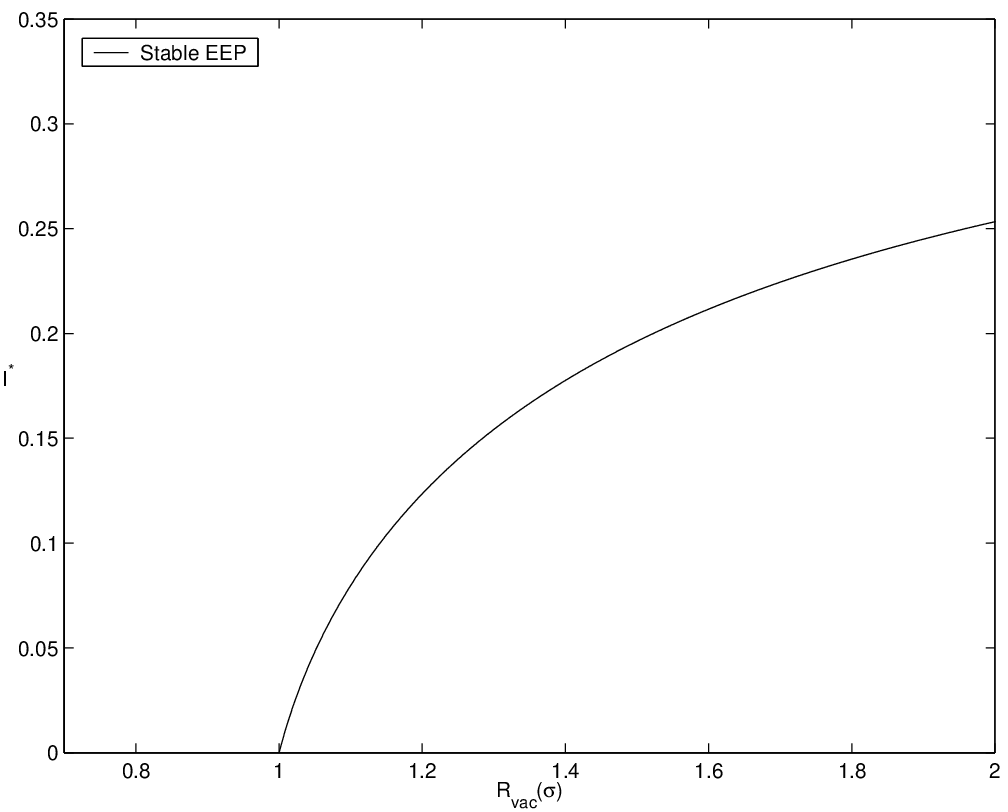
\includegraphics[width=0.7\textwidth]{FIGS/SIRV_bif_forward}
\end{frame}

\begin{frame}{What can happen with vaccination -- Backward bifurcation}
\centering
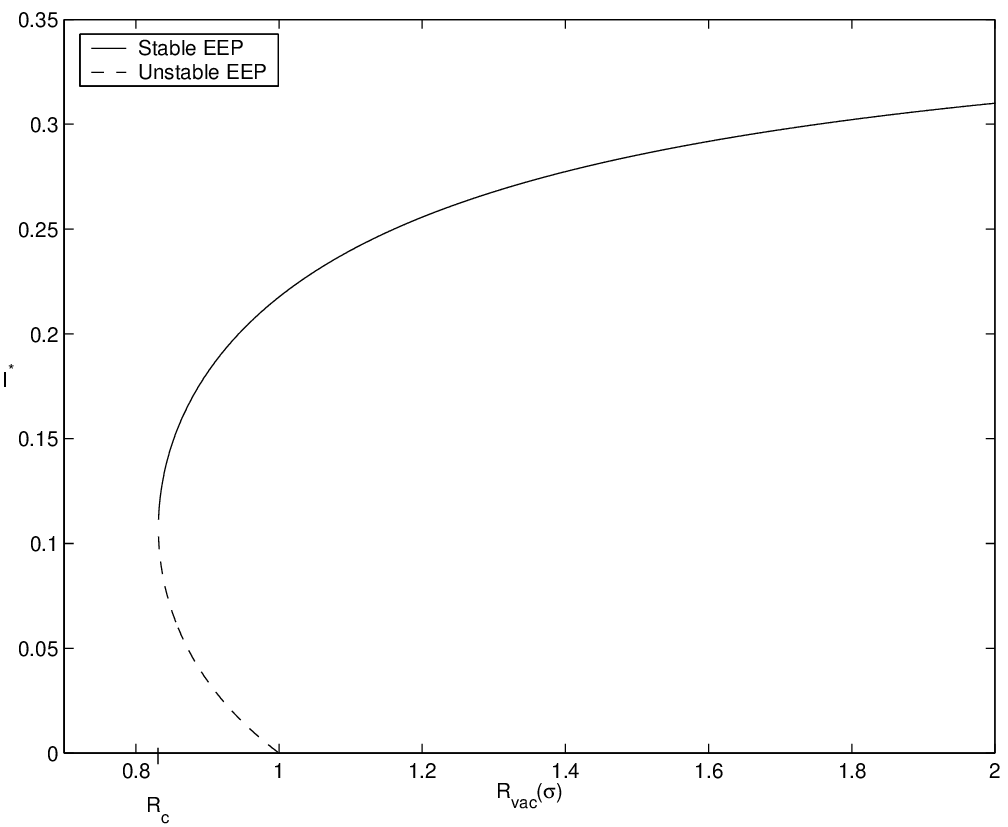
\includegraphics[width=0.7\textwidth]{FIGS/SIRV_bif_backward}
\end{frame}


%%%%%%%%%%%%%%%%%%%%
%%%%%%%%%%%%%%%%%%%%
%%%%%%%%%%%%%%%%%%%%
%%%%%%%%%%%%%%%%%%%%
\section{Vector-borne diseases}
%%%%%%%%%%%%%%%%%%%%
%%%%%%%%%%%%%%%%%%%%
\subsection{Two Ross-Macdonald-type models}
\begin{frame}
See, e.g., Simoy \& Aparicio, \href{https://doi.org/10.1016/j.actatropica.2020.105452}{Ross-Macdonald models: Which one should we use?}, \emph{Acta Tropica} (2020)
\vfill
Ross introduced the model in 1911. Later ``tweaked'' by Macdonald to include mosquito latency period
\vfill
Here, I show a version in the paper cited, with some notation changed
\end{frame}

\begin{frame}
\centering
\resizebox{\textwidth}{!}{
  \def\horskip{*2}
  \def\verskip{*2}
  \begin{tikzpicture}[%transform canvas={scale=1.3},
      auto,
      cloud/.style={minimum width={width("N-1")+2pt},
      draw, 
      ellipse,
      fill=gray!20}]
    %% Hosts
    \node [cloud, fill=green!50] at (0,0) (SH) {$S_H$};
    \node [cloud, fill=red!50] at (1\horskip,0) (IH) {$I_H$};
    \node [cloud, fill=blue!50] at (2\horskip,0) (RH) {$R_H$};
    %% Vectors
    \node [cloud, fill=green!50] at (0,-1\verskip) (SV) {$S_V$};
    \node [cloud, fill=red!50] at (1\horskip,-1\verskip) (IV) {$I_V$};
    %% Births
    \node [left=0.75cm of SH] (birthH) {};
    \node [left=0.75cm of SV] (birthV) {};
    %% Deaths
    \node [below=0.25\verskip of SH] (dSH) {};
    \node [below=0.25\verskip of IH] (dIH) {};
    \node [below=0.25\verskip of RH] (dRH) {};
    \node [below=0.25\verskip of SV] (dSV) {};
    \node [below=0.25\verskip of IV] (dIV) {};
    %%
    \path [line, very thick] (SH) to node [midway,above,sloped] (TextNode) {$\beta_HI_V\frac{S_H}{H}$} (IH);
    \path [line, very thick] (IH) to node [midway,above,sloped] (TextNode) {$\gamma_H I_H$} (RH);
    \path [line, very thick] (SV) to node [midway,below,sloped] (TextNode) {$\beta_VS_V\frac{I_H}{H}$} (IV);
    \path [line, dotted, very thick] (IV) to node [midway,below,sloped] (TextNode) {} (SH);
    \path [line, dotted, very thick] (IH) to node [midway,above,sloped] (TextNode) {} (SV);
    %% Demography
    \path [line, very thick] (birthH) to node [midway,above] (TextNode) {$b_H$} (SH);
    \path [line, very thick] (birthV) to node [midway,above] (TextNode) {$b_V$} (SV);
    \path [line, very thick] (SH) to node [near end,left] (TextNode) {$d_HS_H$} (dSH);
    \path [line, very thick] (IH) to node [near end,right] (TextNode) {$d_HI_H$} (dIH);
    \path [line, very thick] (RH) to node [near end,right] (TextNode) {$d_HR_H$} (dRH);
    \path [line, very thick] (SV) to node [near end,left] (TextNode) {$d_VS_V$} (dSV);
    \path [line, very thick] (IV) to node [near end,right] (TextNode) {$d_VI_V$} (dIV);
  \end{tikzpicture}
}
\end{frame}

\begin{frame}{Reproduction number}
\begin{equation}\label{eq:vector_host_1}
\R_0 =
\frac{\beta_H\beta_V}{(\gamma_H+\gamma_V)d_V}\
\frac{V^\star}{H^\star}
\end{equation}
where $H^\star$ and $V^\star$ are the total host and vector populations, respectively
\end{frame}


\begin{frame}
\centering
\resizebox{\textwidth}{!}{
  \def\horskip{*2}
  \def\verskip{*2}
  \begin{tikzpicture}[%transform canvas={scale=1.3},
      auto,
      cloud/.style={minimum width={width("N-1")+2pt},
      draw, 
      ellipse,
      fill=gray!20}]
    %% Hosts
    \node [cloud, fill=green!50] at (0,0) (SH) {$S_H$};
    \node [cloud, fill=red!10] at (1\horskip,0) (LH) {$L_H$};
    \node [cloud, fill=red!50] at (2\horskip,0) (IH) {$I_H$};
    \node [cloud, fill=blue!50] at (3\horskip,0) (RH) {$R_H$};
    %% Vectors
    \node [cloud, fill=green!50] at (0,-1\verskip) (SV) {$S_V$};
    \node [cloud, fill=red!10] at (1\horskip,-1\verskip) (LV) {$L_V$};
    \node [cloud, fill=red!50] at (2\horskip,-1\verskip) (IV) {$I_V$};
    %% Births
    \node [left=0.75cm of SH] (birthH) {};
    \node [left=0.75cm of SV] (birthV) {};
    %% Deaths
    \node [above=0.5\verskip of SH] (dSH) {};
    \node [above=0.5\verskip of LH] (dLH) {};
    \node [above=0.5\verskip of IH] (dIH) {};
    \node [above=0.5\verskip of RH] (dRH) {};
    \node [below=0.5\verskip of SV] (dSV) {};
    \node [below=0.5\verskip of LV] (dLV) {};
    \node [below=0.5\verskip of IV] (dIV) {};
    %%
    \path [line, very thick] (SH) to node [midway,above,sloped] (TextNode) {$\beta_HI_V\frac{S_H}{H}$} (LH);
    \path [line, very thick] (LH) to node [midway,above,sloped] (TextNode) {$\varepsilon_H L_H$} (IH);
    \path [line, very thick] (IH) to node [midway,above,sloped] (TextNode) {$\gamma_H I_H$} (RH);
    \path [line, very thick] (SV) to node [midway,below,sloped] (TextNode) {$\beta_VS_V\frac{I_H}{H}$} (LV);
    \path [line, very thick] (LV) to node [midway,below,sloped] (TextNode) {$\varepsilon_V L_V$} (IV);
    \path [line, dotted, very thick] (IV) to node [midway,below,sloped] (TextNode) {} (SH);
    \path [line, dotted, very thick] (IH) to node [midway,above,sloped] (TextNode) {} (SV);
    %% Demography
    \path [line, very thick] (birthH) to node [midway,above] (TextNode) {$b_H$} (SH);
    \path [line, very thick] (birthV) to node [midway,above] (TextNode) {$b_V$} (SV);
    \path [line, very thick] (SH) to node [near end,right] (TextNode) {$d_HS_H$} (dSH);
    \path [line, very thick] (LH) to node [near end,right] (TextNode) {$d_HL_H$} (dLH);
    \path [line, very thick] (IH) to node [near end,right] (TextNode) {$d_HI_H$} (dIH);
    \path [line, very thick] (RH) to node [near end,right] (TextNode) {$d_HR_H$} (dRH);
    \path [line, very thick] (SV) to node [near end,right] (TextNode) {$d_VS_V$} (dSV);
    \path [line, very thick] (LV) to node [near end,right] (TextNode) {$d_VL_V$} (dLV);
    \path [line, very thick] (IV) to node [near end,right] (TextNode) {$d_VI_V$} (dIV);
  \end{tikzpicture}
}
\end{frame}

\begin{frame}{Reproduction number}
\begin{equation}\label{eq:vector_host_2}
\R_0 =
\frac{\beta_H\beta_V}{(\gamma_H+\gamma_V)d_V}\
\frac{\varepsilon_V}{d_V+\varepsilon_V}\
\frac{\varepsilon_H}{d_H+\varepsilon_H}\
\frac{V^\star}{H^\star}
\end{equation}
where $H^\star$ and $V^\star$ are the total host and vector populations, respectively
\vfill
Here
\[
f_X = \frac{\varepsilon_X}{d_X+\varepsilon_X}
\]
are the fractions of latent individuals (of type $X=\{V,H\}$) who survive the latency period
\end{frame}


%%%%%%%%%%%%%%%%%%%%
%%%%%%%%%%%%%%%%%%%%
\subsection{A little complexification of Ross-Macdonald}

\begin{frame}{Recall this guy?}
\centering
\resizebox{\textwidth}{!}{
  \def\horskip{*2}
  \def\verskip{*2}
  \begin{tikzpicture}[%transform canvas={scale=1.3},
      auto,
      cloud/.style={minimum width={width("N-1")+2pt},
      draw, 
      ellipse,
      fill=gray!20}]
    %% Hosts
    \node [cloud, fill=green!50] at (0,0) (SH) {$S_H$};
    \node [cloud, fill=red!50] at (1\horskip,0) (IH) {$I_H$};
    \node [cloud, fill=blue!50] at (2\horskip,0) (RH) {$R_H$};
    %% Vectors
    \node [cloud, fill=green!50] at (0,-1\verskip) (SV) {$S_V$};
    \node [cloud, fill=red!50] at (1\horskip,-1\verskip) (IV) {$I_V$};
    %% Births
    \node [left=0.75cm of SH] (birthH) {};
    \node [left=0.75cm of SV] (birthV) {};
    %% Deaths
    \node [below=0.25\verskip of SH] (dSH) {};
    \node [below=0.25\verskip of IH] (dIH) {};
    \node [below=0.25\verskip of RH] (dRH) {};
    \node [below=0.25\verskip of SV] (dSV) {};
    \node [below=0.25\verskip of IV] (dIV) {};
    %%
    \path [line, very thick] (SH) to node [midway,above,sloped] (TextNode) {$\beta_HI_V\frac{S_H}{H}$} (IH);
    \path [line, very thick] (IH) to node [midway,above,sloped] (TextNode) {$\gamma_H I_H$} (RH);
    \path [line, very thick] (SV) to node [midway,below,sloped] (TextNode) {$\beta_VS_V\frac{I_H}{H}$} (IV);
    \path [line, dotted, very thick] (IV) to node [midway,below,sloped] (TextNode) {} (SH);
    \path [line, dotted, very thick] (IH) to node [midway,above,sloped] (TextNode) {} (SV);
    %% Demography
    \path [line, very thick] (birthH) to node [midway,above] (TextNode) {$b_H$} (SH);
    \path [line, very thick] (birthV) to node [midway,above] (TextNode) {$b_V$} (SV);
    \path [line, very thick] (SH) to node [near end,left] (TextNode) {$d_HS_H$} (dSH);
    \path [line, very thick] (IH) to node [near end,right] (TextNode) {$d_HI_H$} (dIH);
    \path [line, very thick] (RH) to node [near end,right] (TextNode) {$d_HR_H$} (dRH);
    \path [line, very thick] (SV) to node [near end,left] (TextNode) {$d_VS_V$} (dSV);
    \path [line, very thick] (IV) to node [near end,right] (TextNode) {$d_VI_V$} (dIV);
  \end{tikzpicture}
}
\end{frame}


\begin{frame}{Let us add a few arrows}
\centering
\resizebox{0.8\textwidth}{!}{
  \def\horskip{*2}
  \def\verskip{*2}
  \begin{tikzpicture}[%transform canvas={scale=1.3},
      auto,
      cloud/.style={minimum width={width("N-1")+2pt},
      draw, 
      ellipse,
      fill=gray!20}]
    %% Hosts
    \node [cloud, fill=green!50] at (0,0) (SH) {$S_H$};
    \node [cloud, fill=red!50] at (1\horskip,0) (IH) {$I_H$};
    \node [cloud, fill=blue!50] at (2\horskip,0) (RH) {$R_H$};
    %% Vectors
    \node [cloud, fill=green!50] at (0,-1\verskip) (SV) {$S_V$};
    \node [cloud, fill=red!50] at (1\horskip,-1\verskip) (IV) {$I_V$};
    %% Births
    \node [left=0.75cm of SH] (birthH) {};
    \node [left=0.75cm of SV] (birthV) {};
    %% Deaths
    \node [below=0.25\verskip of SH] (dSH) {};
    \node [below=0.25\verskip of IH] (dIH) {};
    \node [below=0.25\verskip of RH] (dRH) {};
    \node [below=0.25\verskip of SV] (dSV) {};
    \node [below=0.25\verskip of IV] (dIV) {};
    %%
    \path [line, very thick] (SH) to node [midway,above,sloped] (TextNode) {$\Phi_H$} (IH);
    \path [line, very thick] (IH) to node [midway,above,sloped] (TextNode) {$\gamma_H I_H$} (RH);
    \path [line, very thick] (SV) to node [midway,below,sloped] (TextNode) {$\Phi_V$} (IV);
    \path [line, dotted, very thick] (IV) to node [midway,below,sloped] (TextNode) {} (SH);
    \path [line, dotted, very thick] (IH) to node [midway,above,sloped] (TextNode) {} (SV);
    \draw [>=latex,->, thick, rounded corners] (IH) -- (1\horskip,0.75) -- (0,0.75) node[midway,above,sloped] {$\rho_H I_H$} -- (SH);
    \draw [>=latex,->, thick, rounded corners] (RH) -- (2\horskip,1.5) -- (-0.35,1.5) node[midway,above,sloped] {$\nu_H R_H$} -- (SH.north west);
    %% Demography
    \path [line, very thick] (birthH) to node [midway,above] (TextNode) {$b_H$} (SH);
    \path [line, very thick] (birthV) to node [midway,above] (TextNode) {$b_V$} (SV);
    \path [line, very thick] (SH) to node [near end,left] (TextNode) {$d_HS_H$} (dSH);
    \path [line, very thick] (IH) to node [near end,right] (TextNode) {$d_HI_H$} (dIH);
    \path [line, very thick] (RH) to node [near end,right] (TextNode) {$d_HR_H$} (dRH);
    \path [line, very thick] (SV) to node [near end,left] (TextNode) {$d_VS_V$} (dSV);
    \path [line, very thick] (IV) to node [near end,right] (TextNode) {$d_VI_V$} (dIV);
  \end{tikzpicture}
}
\end{frame}

\begin{frame}
Arino, Ducrot \& Zongo, \href{https://julien-arino.github.io/assets/pdf/papers/2012_ArinoDucrotZongo-JMB64.pdf}{A metapopulation model for malaria with transmission-blocking partial immunity in hosts}, Journal of Mathematical Biology (2012)
\vfill
Incidence functions take the form
\[
\Phi_H = b_H(H,V)\sigma_{VH}\frac{I_V}{V}
\]
and 
\[
\Phi_V = b_V(H,V)\left(\sigma_{HV}\frac{I_H}{H}+\hat\sigma_{HV}\frac{R_H}{H}\right)
\]
where $b_{H}$ and $b_V$ are numbers per unit time of mosquito bites a human has and the number of humans a mosquito bites, respectively
\end{frame}

\begin{frame}{Parameters of the incidence function}
\begin{itemize}
\item $\sigma_{HV}$ probability of transmission of the parasite (in gametocyte form) from
an infectious human to a susceptible mosquito
\item $\hat\sigma_{HV}$ probability of transmission of the parasite (in gametocyte form) from
a semi-immune human to a susceptible mosquito
\item $\sigma_{VH}$ probability of transmission of the parasite (in sporozoite form) from
an infectious mosquito to a susceptible human
\end{itemize}
\vfill
Additional parameter that can be factored in (all per unit time)
\begin{itemize}
\item $a_H$ maximum number of mosquito bites a human can receive
\item $a_V$ number of times one mosquito would ``want to'' bite humans
\item $a$ average number of bites given to humans by each mosquito
\end{itemize}
\end{frame}

\begin{frame}{People to read for malaria models (IMOBO)}
See also the work of 
\vfill
\begin{itemize}
\item \href{https://scholar.google.com/citations?user=AwKMfZ8AAAAJ&hl=en}{Gideon Ngwa} at the University of Buea
\vfill
\item \href{https://scholar.google.ch/citations?user=BMiKO0UAAAAJ&hl=en}{Nakul Chitnis} at the Swiss Tropical and Public Health Institute
\end{itemize}
\vfill
Many others...
\end{frame}


\begin{frame}{More complex models may be needed for malaria}
Timing of processes is critical in malaria
\vfill
Plasmodium life cycle in the mosquito is commensurate with mosquito lifetime
\vfill
Need models that are able to account for that, because ODEs are not really good at this (see beginning of Stochastic systems lecture)
\vfill
Mathematics becomes more complicated
\end{frame}

%%%%%%%%%%%%%%%%%%%%
%%%%%%%%%%%%%%%%%%%%
%%%%%%%%%%%%%%%%%%%%
%%%%%%%%%%%%%%%%%%%%
\section{Immunology}

\begin{frame}{Caveat}
I don't know much about this, this past year and a bit is the first time I have worked on this...
\vfill
I recommend reading, e.g., Eftimie, Gillard \& Cantrell, \href{https://doi.org/10.1007/s11538-016-0214-9}{Mathematical Models for Immunology: Current State of the Art and Future Research Directions}, \emph{Bulletin of Mathematical Biology} (2016)
\vfill
Look also at the work of \href{https://scholar.google.com/citations?user=ARpn4H0AAAAJ&hl=en}{Alan Perelson} or read Wodarz's \href{https://doi.org/10.1007/978-0-387-68733-9}{Killer Cell Dynamics} (\href{http://ndl.ethernet.edu.et/bitstream/123456789/23447/1/Dominik\%20Wodarz.pdf}{or here})
\end{frame}

\begin{frame}{A simple model}
State variables
\begin{itemize}
\item susceptible uninfected cells $x$
\item infected cells $y$
\item free virus $v$
\end{itemize}
\vfill
\begin{align*}
x\pprime &= \lambda -dx-\beta xv \\
y\pprime &= \beta xv-ay \\
v\pprime &= ky-uv
\end{align*}
\end{frame}


\begin{frame}{Side note (a.k.a. little rank) -- IMOBO don't do that}
There is a tradition, typically stemming from the British modelling school, to use ``random'' letters for state variables
\vfill
\begin{minipage}{0.45\textwidth}
\begin{align*}
x\pprime &= \lambda -dx-\beta xv \\
y\pprime &= \beta xv-ay \\
v\pprime &= ky-uv
\end{align*}
\end{minipage}
\hfill
\begin{minipage}{0.45\textwidth}
\begin{align*}
S\pprime &= \lambda -dS-\beta SV \\
I\pprime &= \beta SV-aI \\
V\pprime &= kI-uV
\end{align*}
\end{minipage}
\vfill
Modelling is hard enough without needing to recall what $x$, $y$, $z$, etc., stand for
\end{frame}

\begin{frame}
\begin{subequations}
\begin{align}
S\pprime &= \lambda -dS-\beta SV \\
I\pprime &= \beta SV-aI \\
V\pprime &= kI-uV
\end{align}
\end{subequations}
\vfill
Virus-free equilibrium (VFE) $\bE_0=(\lambda/d,0,0)$ and establishment of infection
\[
\bE_\star = \left(\frac{au}{\beta k},\frac{\lambda\beta k-dau}{a\beta k},
\frac{\lambda\beta k-dau}{a\beta u}\right)
\]
\vfill
\[
\R_0 = \frac{\lambda\beta k}{dau}
\]
\end{frame}

\begin{frame}{Simplification}
Free virus population has much faster dynamics that cells, so we can assume virus population is at a quasi-steady state $V=kI/u$ 
\vfill
Mode becomes
\begin{subequations}
\begin{align}
S\pprime &= \lambda -dS-\tilde\beta SI \\
I\pprime &= \tilde\beta SI-aI \\
\end{align}
where
\[
\tilde\beta = \frac{\beta k}{u}
\]
\vfill
Drop the tilde on $\beta$, then 
\[
\R_0=\frac{\beta k}{da}
\]
\end{subequations}
\end{frame}


\begin{frame}{Incorporating CTL dynamics}
CTL proliferate when stimulated by viral antigen
\vfill
\begin{subequations}
\begin{align}
S\pprime &= \lambda-dS-\beta SI \\
I\pprime &= \beta SI-aI-pIC \\
C\pprime &= cIC-bC
\end{align}
\end{subequations}
\vfill
Assume $\R_0>1$, i.e., the virus can successfully establish itself
\vfill
Then if $(\lambda/a-d/\beta)c<d$, the CTL response fails to become established and the system goes to $(\beta/K,\lambda/K-d/\beta,0)$
\vfill
If $(\lambda/a-d/\beta)c>d$, then the system converges to
\[
\left(
\frac{\lambda c}{dc+\beta b},\frac bc,
\frac{(\beta\lambda-ad)c-ab\beta}{(cd+\beta b)p}
\right)
\]
\end{frame}
%%%%%%%%%%%%%%%%%%%%
%%%%%%%%%%%%%%%%%%%%
%%%%%%%%%%%%%%%%%%%%
%%%%%%%%%%%%%%%%%%%%
\section{A few other models}
%%%%%%%%%%%%%%%%%%%%
%%%%%%%%%%%%%%%%%%%%
\subsection{A model of Capasso for ETP}

\begin{frame}{A minimal model of V. Capasso}
  \begin{center}
    \def\vertskip{*1.75}
    \def\horzskip{*2}
    \begin{tikzpicture}[scale=1.5, transform shape]
      \node [circle, fill=gray!10, text=black] at (-1\horzskip,0\vertskip) (H) {$H$};
      \node [circle, fill=gray!10, text=black] at (1\horzskip,0\vertskip) (E) {$E$};
      %% Flows between
      \path [line, very thick, bend left] (H) to node [near end, above] (TextNode) {$c_HH$} (E);
      \path [line, very thick, bend left] (E) to node [near end, below] (TextNode) {$g(E)$} (H);
      %% Flows out of
      \path [line, very thick] (H) to node [midway, above] (TextNode) {$\gamma_HH$} (-1.75\horzskip,0\vertskip);
      \path [line, very thick] (E) to node [midway, below] (TextNode) {$d_EE$} (1.75\horzskip,0\vertskip);
      %% Vertical line
      \draw [dashed, very thick, color=red] (0\horzskip,-1\vertskip) -- (0\horzskip,1\vertskip);
      %% Text
      \node [color=red] at (-1\horzskip,-1\vertskip) {Human population};
      \node [color=red] at (1\horzskip,-1\vertskip) {Environment};
    \end{tikzpicture}    
  \end{center}  
  $1/\gamma_H$ mean infectious period, $1/d_E$ mean lifetime of the agent in the environment, $c_H$ growth rate of the agent due to the human population, $g(E)$ ``force of infection'' (I would say ``incidence'') of the agent on human population
\end{frame}

\begin{frame}{Incidence function}
  \begin{equation}
    \label{eq:incidence_function_Capasso}
    g(E) = N\beta ph(E)
  \end{equation}
  where
  \begin{itemize}
    \item $N$ total human population
    \item $\beta$ fraction of susceptible individuals in $N$
    \item $p$ fraction exposed to contaminated environment per unit time (``probability per unit time to have a ``snack'' of contaminated food'')
    \item $h(E)$ probability for an exposed susceptible to get the infection
  \end{itemize}
  Typically, we would assume $p$ and $\beta$ independent of $E$ and $H$ and $h$ to be saturating
\end{frame}

\begin{frame}
  To ensure \eqref{eq:incidence_function_Capasso} satisfies these conditions, we can assume
  \begin{itemize}
    \item $0<g(e_1)<g(e_2)$ for $0<e_1<e_2$
    \item $g(0)=0$
    \item $g''(z)<0$ for all $z>0$
    \item $0<g'_+(0)<\infty$  (right derivative)
    \item $\lim_{z\to\infty}\frac{g(z)}{z}<\frac{d_E\gamma_H}{c_H}$
  \end{itemize}
  \vfill
  Of course, we also assume $d_E,c_H,\gamma_H>0$
\end{frame}

\begin{frame}{The model}
  \begin{subequations}
    \label{sys:capasso_EH}
    \begin{align}
      E\pprime &= c_HH-d_EE \label{sys:capasso_EH_dE} \\
      H\pprime &= g(E)-\gamma_HH \label{sys:capasso_EH_dH}
    \end{align}
  \end{subequations}
  \begin{center}
    \def\vertskip{*1.75}
    \def\horzskip{*2}
    \begin{tikzpicture}[scale=1, transform shape]
      \node [circle, fill=gray!10, text=black] at (-1\horzskip,0\vertskip) (H) {$H$};
      \node [circle, fill=gray!10, text=black] at (1\horzskip,0\vertskip) (E) {$E$};
      %% Flows between
      \path [line, very thick, bend left] (H) to node [near end, above] (TextNode) {$c_HH$} (E);
      \path [line, very thick, bend left] (E) to node [near end, below] (TextNode) {$g(E)$} (H);
      %% Flows out of
      \path [line, very thick] (H) to node [midway, above] (TextNode) {$\gamma_HH$} (-1.75\horzskip,0\vertskip);
      \path [line, very thick] (E) to node [midway, below] (TextNode) {$d_EE$} (1.75\horzskip,0\vertskip);
      %% Vertical line
      \draw [dashed, very thick, color=red] (0\horzskip,-1\vertskip) -- (0\horzskip,1\vertskip);
      %% Text
      \node [color=red] at (-1\horzskip,-1\vertskip) {Human population};
      \node [color=red] at (1\horzskip,-1\vertskip) {Environment};
    \end{tikzpicture}    
  \end{center}
  \vfill
  Pay attention to the flows..! $E\pprime$ does not have a $-g(E)$ and $H\pprime$ does not have $-c_HH$. Why?
\end{frame}

\begin{frame}
  Let
  \begin{equation}
    \label{eq:R0_capasso}
    \R_0 = \frac{g'_+(0)c_H}{d_E\gamma_H}
  \end{equation}
  \begin{theorem}
    \begin{itemize}
      \item If $0<\R_0<1$, then \eqref{sys:capasso_EH} admits only the trivial equilibrium in the positive orthant, which is GAS
      \item If $\R_0>1$, then two EP exist: $(0,0)$, which is unstable, and $z^\star=(E^\star,H^\star)$ with $E^\star,H^\star>0$, GAS in $\IR_+^2\setminus\{0,0\}$
    \end{itemize}
  \end{theorem}
\end{frame}


\begin{frame}{Adding a periodic component}
  Assume $p$ in \eqref{eq:incidence_function_Capasso} takes the form 
  \begin{equation}
    p(t)=p(t+\omega)>0,\quad t\in\IR
  \end{equation}
  i.e., $p$ has period $\omega$. So we now consider the incidence
  \begin{equation}
    \label{eq:incidence_Capasso_periodic}
    g(t,E)=p(t)h(E)
  \end{equation}
  with $h$ having the properties prescribed earlier.
  Letting 
  \begin{equation}
    p_{min} := \min_{0\leq t\leq\omega}p(t),\quad
    p_{max} := \max_{0\leq t\leq\omega}p(t)
  \end{equation}
  then we require that 
  \begin{equation}
    \lim_{z\to\infty}\frac{g(z)}{z}<\frac{d_E\gamma_H}{c_Hp_{max}}
  \end{equation}
\end{frame}


\begin{frame}
  Let
  \begin{equation}
    \label{eq:R0_capasso_periodic}
    \R_0^{min} = \frac{c_Hp_{min}h'_+(0)}{d_E\gamma_H},\quad 
    \R_0^{max} = \frac{c_Hp_{max}h'_+(0)}{d_E\gamma_H}
  \end{equation}
  \begin{theorem}
    \begin{itemize}
      \item If $0<\R_0^{max}<1$, then \eqref{sys:capasso_EH} with incidence \eqref{eq:incidence_Capasso_periodic} always goes to extinction
      \item If $\R_0^{min}>1$, then a unique nontrivial periodic endemic state exists for \eqref{sys:capasso_EH} with incidence \eqref{eq:incidence_Capasso_periodic}
    \end{itemize}
  \end{theorem}
\end{frame}

\begin{frame}[fragile]{Simulating (in \code{R}) -- Incidence function}
\begin{lstlisting}
h = function(E, params) {
  # Use Michaelis Menten (Holling type II) growth
  OUT = params$g_max * E / (params$g_half+E)
  return(OUT)
}
g = function(E, params) {
  OUT = params$N * params$beta * params$p * h(E,params)
  return(OUT)
}
\end{lstlisting}
\end{frame}

\begin{frame}[fragile]{The right hand side}
\begin{lstlisting}
rhs_Capasso_ODE = function(t, x, params) {
  with(as.list(c(x, params)), {
    dE = c_H*H-d_E*E
    dH = g(E, params)-gamma_H*H
    list(c(dE, dH))
  })
}  
\end{lstlisting}
\end{frame}

\begin{frame}[fragile]{Setting parameters}
\begin{lstlisting}
# Put parameters in a list
params = list()
params$N = 1000       # Total population
params$gamma_H = 1/10 # Infectious period
params$d_E = 1/5      # Lifetime agent
params$c_H = 0.1      # Flow from humans
# Human characteristics and behaviour
params$beta = 0.2 # Fraction susceptible
params$p = 0.1    # Probability of having "snack"
# Growth function
params$g_max = 10
params$g_half = 100
# Final time
params$t_f = 150  
\end{lstlisting}
\end{frame}

\begin{frame}[fragile]{Running and plotting (base)}
\begin{lstlisting}
IC <- c(E = 10, H = 0)
tspan = seq(from = 0, to = params$t_f, by = 0.1)

sol_ODE = ode(y = IC,
              func = rhs_Capasso_ODE,
              times = tspan,
              parms = params)

plot(sol_ODE[,"time"], sol_ODE[,"H"],
      type = "l", lwd = 2,
      xlab = "Time (days)", ylab = "Value")
lines(sol_ODE[,"time"], sol_ODE[,"E"], 
      lwd = 2, lty = 3)
legend("bottomright", legend = c("H(t)", "E(t)"),
        lwd = c(2,2), lty = c(1,3), inset = 0.01)
\end{lstlisting}
\end{frame}


\begin{frame}
  \begin{center}
    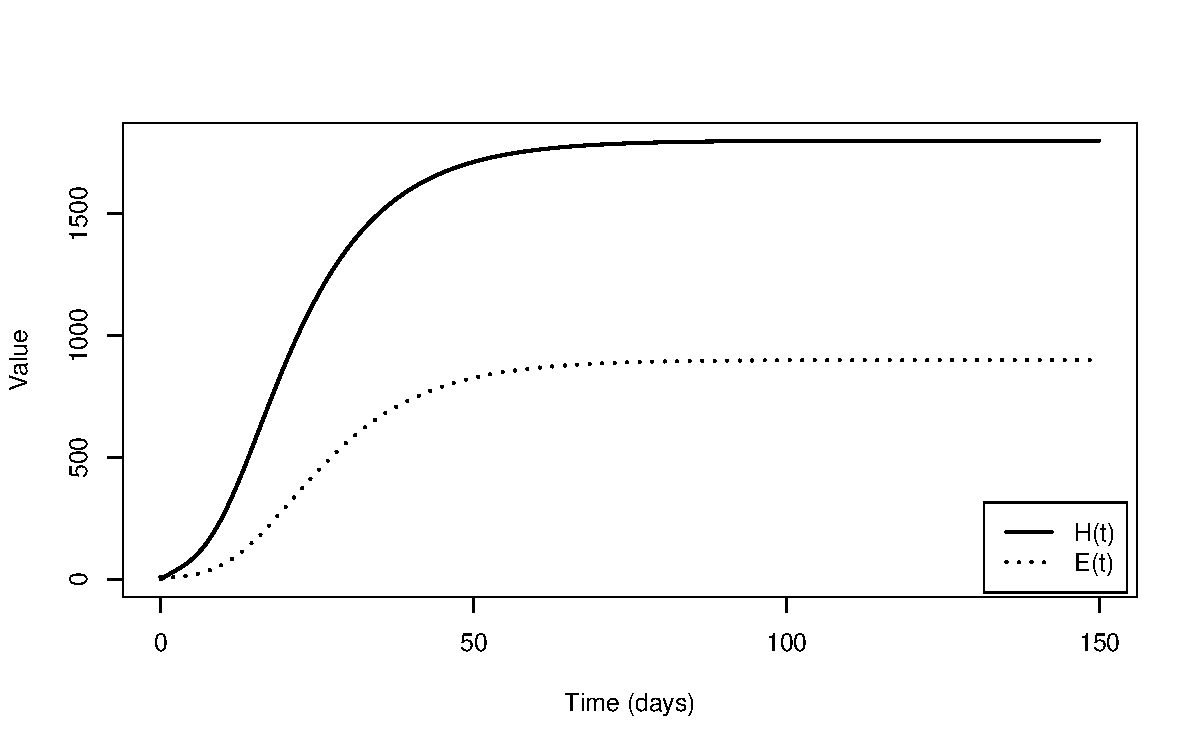
\includegraphics[width=\textwidth]{FIGS/lecture-02-Capasso_ETP_1}
  \end{center}
\end{frame}

\begin{frame}
  Let
  \begin{equation}
    \tag{\ref{eq:R0_capasso}}
    \R_0 = \frac{g'_+(0)c_H}{d_E\gamma_H}
  \end{equation}
  \begin{theorem}
    \begin{itemize}
      \item If $0<\R_0<1$, then \eqref{sys:capasso_EH} admits only the trivial equilibrium in the positive orthant, which is GAS
      \item If $\R_0>1$, then two EP exist: $(0,0)$, which is unstable, and $z^\star=(E^\star,H^\star)$ with $E^\star,H^\star>0$, GAS in $\IR_+^2\setminus\{0,0\}$
    \end{itemize}
  \end{theorem}
\end{frame}

\begin{frame}[fragile]{Computing $\R_0$}
  With the chosen $g$, we have
  \[
    g'(E) = 
    \frac{N \beta pg_{half} g_{max}}
    {(g_{half}+E)^2}
  \]
  whence
  \[
    g_+'(0)=\frac{N \beta pg_{max}}
    {g_{half}}
  \]
  and thus
  \begin{equation}
    \R_0 = \frac{N \beta pg_{max}}
    {g_{half}}\;\frac{c_H}{d_E\gamma_H}
  \end{equation}
\begin{lstlisting}
R0 = function(params) {
  with(as.list(params), {
    R0 = N*beta*p*g_max*c_H / (g_half*d_E*gamma_H)
    return(R0)
  })
}  
\end{lstlisting}
\end{frame}


\begin{frame}{Showing things dynamically using Shiny}
  Shiny is an \code{R} library (made by RStudio) to easily make interactive displays
  \vfill
  See some documentation \href{https://shiny.rstudio.com/}{here}
  \vfill
  Some examples \href{https://shiny.rstudio.com/gallery/}{here} and \href{https://github.com/rstudio/shiny-examples}{here}
  \vfill
  Create a subdirectory with the name of your app and a file called \code{app.R} in there
\end{frame}


\begin{frame}{Structure of a Shiny app}
  Need to use library \code{shiny}
  \vfill
  Define two elements
  \begin{itemize}
    \item \code{ui}, which sets up the user interface
    \item \code{server}, which handles the computations, generation of figures, etc.
  \end{itemize}
  \vfill
  I explain different elements as we progress. See the code in the \code{CODE} folder and \code{Capasso\_simpleETP\_shiny} subdirectory
\end{frame}


\begin{frame}[fragile]{The \code{ui} part}
Here, we use \code{fluidPage} to create the UI. There are other functions: \code{fillPage}, \code{fixedPage}, \code{flowLayout}, \code{navbarPage}, \code{sidebarLayout}, \code{splitLayout} and \code{verticalLayout}
\vfill
\begin{lstlisting}
# Define UI
ui <- fluidPage(
)  
\end{lstlisting}
\vfill
We now fill this function
\end{frame}

\begin{frame}[fragile]{A title and some sliders}
\begin{lstlisting}
# Application title
titlePanel("Simple ETP model of Capasso"),
# Sidebar with slider inputs for some parameters
sidebarLayout(
    sidebarPanel(
      sliderInput("inv_gamma_H",
                  "Average infectious period (days):",
                  min = 0,
                  max = 30,
                  value = 10),
      sliderInput("c_H",
                  "Flow from humans:",
                  min = 0,
                  max = 2,
                  value = 0.1),
\end{lstlisting}
\vfill
Plus other sliders for all other parameters
\end{frame}

\begin{frame}[fragile]{Note the little trick...}
\begin{lstlisting}
sliderInput("inv_gamma_H",
"Average infectious period (days):",
min = 0,
max = 30,
value = 10),
\end{lstlisting}
\vfill
I want to give a user friendly version of the parameter value, using the number of days rather than the inverse, whereas the model uses the latter. So I prefix the variable name by \code{inv\_} and then process as follows in the \code{server} part
\begin{lstlisting}
params <- list()
for (param_name in names(input)) {
  if (grepl("inv_", param_name)) {
    new_param_name = gsubs("inv_", "", param_name)
    params[[new_param_name]] = 1/input[[param_name]]
  } else {
    params[[param_name]] = input[[param_name]]
  }
}
\end{lstlisting}
\end{frame}

\begin{frame}
  The simulation functions can be outside of \code{ui} or \code{server}, this makes the code neater
  \vfill
  These functions are the same as before (right hand side, g, h, R0), so they are not shown here
\end{frame}
    

\begin{frame}[fragile]{The \code{server} part}
\begin{lstlisting}
# Define server logic required to draw the result
server <- function(input, output) {
  ##
  ## Expression that generates the plot
  ##
  output$a_odePlot <- renderPlot({
    params <- list()
    params$N = 1000 # We could let this vary, we don't here..
    for (param_name in names(input)) {
      if (grepl("inv_", param_name)) {
        new_param_name = gsub("inv_", "", param_name)
        params[[new_param_name]] = 1/input[[param_name]]
      } else {
        params[[param_name]] = input[[param_name]]
      }
    }
    # Initial conditions and time span
    IC <- c(E = 10, H = 0)
    tspan <- seq(from = 0, to = params$tf, by = 0.1)  
\end{lstlisting}
\end{frame}
  

\begin{frame}[fragile]{The \code{server} part (continued)}
\begin{lstlisting}
    # Compute solution
    sol_ODE = ode(y = IC,
                  func = rhs_Capasso_ODE,
                  times = tspan,
                  parms = params)
    # Make the plot
    y_max = max(max(sol_ODE[,"H"]),sol_ODE[,"E"])
    plot(sol_ODE[,"time"], sol_ODE[,"H"],
          type = "l", lwd = 2,
          xlab = "Time (days)", ylab = "Value",
          ylim = c(0, y_max),
          main = sprintf("R_0=%1.2f", round(R0(params),2)))
    lines(sol_ODE[,"time"], sol_ODE[,"E"], 
          lwd = 2, lty = 3)
    legend("topleft", legend = c("H(t)", "E(t)"),
            lwd = c(2,2), lty = c(1,3), inset = 0.01)
  })
}
\end{lstlisting}
\end{frame}

\begin{frame}[fragile]{Finally, run the code}
\begin{lstlisting}
# Run the application 
shinyApp(ui = ui, server = server)
\end{lstlisting}
\end{frame}
  

\begin{frame}{Adding a periodic component}
  Assume $p$ in \eqref{eq:incidence_function_Capasso} takes the form 
  \begin{equation}
    p(t)=p(t+\omega)>0,\quad t\in\IR
  \end{equation}
  i.e., $p$ has period $\omega$. So we now consider the incidence
  \begin{equation}
    \tag{\ref{eq:incidence_Capasso_periodic}}
    g(t,E)=p(t)h(E)
  \end{equation}
  with $h$ having the properties prescribed earlier.
  Letting 
  \begin{equation}
    p_{min} := \min_{0\leq t\leq\omega}p(t),\quad
    p_{max} := \max_{0\leq t\leq\omega}p(t)
  \end{equation}
  then we require that 
  \begin{equation}
    \lim_{z\to\infty}\frac{g(z)}{z}<\frac{d_E\gamma_H}{c_Hp_{max}}
  \end{equation}
\end{frame}


\begin{frame}
  Let
  \begin{equation}
    \tag{\ref{eq:R0_capasso_periodic}}
    \R_0^{min} = \frac{c_Hp_{min}h'_+(0)}{d_E\gamma_H},\quad 
    \R_0^{max} = \frac{c_Hp_{max}h'_+(0)}{d_E\gamma_H}
  \end{equation}
  \begin{theorem}
    \begin{itemize}
      \item If $0<\R_0^{max}<1$, then \eqref{sys:capasso_EH} with incidence \eqref{eq:incidence_Capasso_periodic} always goes to extinction
      \item If $\R_0^{min}>1$, then a unique nontrivial periodic endemic state exists for \eqref{sys:capasso_EH} with incidence \eqref{eq:incidence_Capasso_periodic}
    \end{itemize}
  \end{theorem}
\end{frame}

\begin{frame}[fragile]{How to add periodicity in numerics?}
\begin{lstlisting}
p_t = function(t, params) {
  angle = 2*pi/params$p_period
  OUT = cos(angle*t) # Make the base cos wave
  OUT = OUT/2*(params$p_max-params$p_min) # Scale
  OUT = OUT-min(OUT)+params$p_min # Shift up
  return(OUT)
}   
g = function(E, params, t) {
  OUT = params$N * params$beta * p_t(t, params) * h(E,params)
  return(OUT)
}
R0 = function(params) {
  with(as.list(params), {
    R0 = list()
    R0$min = N*beta*p_min*g_max*c_H / (g_half*d_E*gamma_H)
    R0$max = N*beta*p_max*g_max*c_H / (g_half*d_E*gamma_H)
    return(R0)
  })
}  
\end{lstlisting}
\end{frame}


%%%%%%%%%%%%%%%%%%%%
%%%%%%%%%%%%%%%%%%%%
\subsection{A model for zoonotic transmission of waterborne disease}

\begin{frame}{Zoonotic transmission of waterborne disease}
Waters, Hamilton, Sidhu, Sidhu \& Dunbar, \href{https://doi-org.uml.idm.oclc.org/10.1007/s11538-015-0136-y}{Zoonotic transmission of waterborne disease: a mathematical model},  \emph{Bull Math Biol}  (2016)
\vfill
Used for instance to model Giardia transmission from possums to humans
\end{frame}

\begin{frame}
  \begin{center}
    \def\vertskip{*2}
    \def\horzskip{*3}
    \begin{tikzpicture}[scale=1, transform shape]
      \node [rectangle, fill=gray!10, text=black] at (-1\horzskip,0\vertskip) (S_H) {Susceptible humans};
      \node [rectangle, fill=gray!10, text=black] at (1\horzskip,0\vertskip) (I_H) {Infectious humans};
      \node [rectangle, fill=gray!10, text=black] at (-1\horzskip,2\vertskip) (S_A) {Susceptible animals};
      \node [rectangle, fill=gray!10, text=black] at (1\horzskip,2\vertskip) (I_A) {Infectious animals};
      \node [rectangle, fill=gray!10, text=black] at (0\horzskip,1\vertskip) (W) {Live oo/cysts in water};
      %% Flows 
      \path [line, very thick] (S_H.south east) to node [midway, below] (TextNode) {P2P transmission} (I_H.south west);
      \path [line, dashed, very thick] (S_H.north east) to node [near end, above] (TextNode) {conversion of oo/cysts to infection} (I_H.north west);
      \path [line, very thick, bend left] (I_H) to node [midway, below] (TextNode) {recovery} (S_H);
      \path [line, very thick] (S_A.north east) to node [midway, above] (TextNode) {A2A transmission} (I_A.north west);
      \path [line, very thick] (I_A.south west) to node [midway, below] (TextNode) {recovery} (S_A.south east);
      %% Flows of W
      \path [line, dashed, very thick] (W) to node [midway, above] (TextNode) {Death of oo/cysts in water} (-2\horzskip,1\vertskip);
      \path [line, dashed, very thick] (W) to node [near start, left] (TextNode) {pick up rate} (0\horzskip,0.35\vertskip);
      \path [line, dashed, very thick] (I_A) to node [midway, below] (TextNode) {deposit rate} (W);
    \end{tikzpicture}    
  \end{center}  
\end{frame}

\begin{frame}
  \begin{center}
    \def\vertskip{*2}
    \def\horzskip{*2}
    \begin{tikzpicture}[scale=1.25, transform shape]
      \node [circle, fill=gray!10, text=black] at (-1\horzskip,0\vertskip) (S_H) {$S_H$};
      \node [circle, fill=gray!10, text=black] at (1\horzskip,0\vertskip) (I_H) {$I_H$};
      \node [circle, fill=gray!10, text=black] at (-1\horzskip,2\vertskip) (S_A) {$S_A$};
      \node [circle, fill=gray!10, text=black] at (1\horzskip,2\vertskip) (I_A) {$I_A$};
      \node [circle, fill=gray!10, text=black] at (0\horzskip,1\vertskip) (W) {$W$};
      %% Flows between
      \path [line, very thick] (S_H) to node [midway, below] (TextNode) {$\beta_H$} (I_H);
      \path [line, dashed, very thick, bend left] (S_H) to node [near end, above] (TextNode) {$\rho$} (I_H);
      \path [line, very thick, bend left] (I_H) to node [midway, below] (TextNode) {$\gamma_HI_H$} (S_H);
      \path [line, very thick, bend left] (S_A) to node [midway, above] (TextNode) {$\beta_A$} (I_A);
      \path [line, very thick, bend left] (I_A) to node [midway, above] (TextNode) {$\gamma_AI_A$} (S_A);
      %% Flows of W
      \path [line, dashed, very thick] (W) to node [midway, above] (TextNode) {$\mu W$} (-0.75\horzskip,1\vertskip);
      \path [line, dashed, very thick] (W) to node [near start, left] (TextNode) {$\eta$} (0\horzskip,0.35\vertskip);
      \path [line, dashed, very thick] (I_A) to node [midway, below, sloped] (TextNode) {$\alpha I_A$} (W);
    \end{tikzpicture}    
  \end{center}  
\end{frame}


\begin{frame}{The full model}
  \begin{subequations}
    \label{sys:WaterHamilton_etal}
    \begin{align}
      S_A\pprime &= -\beta_AS_AI_A+\gamma_AI_A \\
      I_A\pprime &= \beta_AS_AI_A-\gamma_AI_A \\
      W\pprime &= \alpha I_A-\eta W(S_H+I_H)-\mu W \\
      S_H\pprime &= -\rho\eta WS_H-\beta_HS_HI_H+\gamma_HI_H \\
      I_H\pprime &= \rho\eta WS_H+\beta_HS_HI_H-\gamma_HI_H 
    \end{align}
  \end{subequations}
  \vfill
  Considered with $N_A=S_A+I_A$ and $N_H=S_H+I_H$ constant
\end{frame}

\begin{frame}{Simplified model}
  Because $N_A$ and $N_H$ are constant, \eqref{sys:WaterHamilton_etal} can be simplified:
  \begin{subequations}
    \label{sys:WaterHamilton_etal_simplified}
    \begin{align}
      I_A\pprime &= \beta_AN_AI_A-\gamma_AI_A-\beta_AI_A^2 \\
      W\pprime &= \alpha I_A-\eta WN_H-\mu W \\
      I_H\pprime &= \rho\eta W(N_H-I_H)+\beta_HN_HI_H-\gamma_HI_H-\beta_HI_H^2 
    \end{align}
  \end{subequations}
  \vfill
  Three EP: DFE $(0,0,0)$; endemic disease in humans because of H2H transmission; endemic in both H and A because of W
\end{frame}


\begin{frame}
  Three EP: DFE $(0,0,0)$; endemic disease in humans because of H2H transmission; endemic in both H and A because of W
  \vfill
  Let
  \begin{equation}
    \R_{0A} = \frac{\beta_A}{\gamma_A}N_A\quad\text{and}\quad
    \R_{0H} = \frac{\beta_H}{\gamma_H}N_H
  \end{equation}
  \vfill
  \begin{itemize}
    \item DFE LAS if $\R_{0A}<1$ and $\R_{0H}<1$, unstable if $\R_{0A}>1$ or $\R_{0H}>1$
    \item If $\R_{0H}>1$ and $\R_{0A}<1$, \eqref{sys:WaterHamilton_etal_simplified} goes to EP with endemicity only in humans
    \item Endemic EP with both A and H requires $\R_{0A}>1$ and $\R_{0H}<1$
  \end{itemize}
  Note that proof is \textbf{not} global
\end{frame}

%%%%%%%%%%%%%%%%%%%%
%%%%%%%%%%%%%%%%%%%%
\subsection{A few models of schistosomiasis}

%%%%%%%%%%%%%%%%%%%%
%%%%%%%%%%%%%%%%%%%%
\subsubsection{A first model of Woolhouse}
\begin{frame}{A model of Woolhouse}
  Woolhouse. \href{}{On the application of mathematical models of schistosome transmission dynamics. I. Natural transmission}. \emph{Acta Tropica} \textbf{49}:241-270 (1991)
\end{frame}

\begin{frame}{The model}
  Population of $H$ individuals using a body of water containing $N$ snails
  \vfill
  $i_H$ mean number of schistosomes per person and $i_S$ the proportion of patent infections in snails 
  (prevalence)
  \vfill
  \begin{subequations}
    \label{sys:Woolhouse}
    \begin{align}
      i_H\pprime &= \alpha Ni_S-\gamma i_H \\
      i_S\pprime &= \beta Hi_H(1-i_S)-\mu_2 i_S
    \end{align}
  \end{subequations}
  \begin{itemize}
    \item $\alpha$ number of schistosomes produced per person per infected snail per unit time
    \item $1/\gamma$ average life expectancy of a schistosome
    \item $1/\mu_2$ average life expectancy of an infected snail
    \item $\beta$ transmission parameter
  \end{itemize}
\end{frame}

\begin{frame}
  Let the basic reproductive rate for schistosomes be
  \begin{equation}
    \label{eq:R0_Woolhouse}
    \R_0 = \frac{\alpha N\beta H}{\gamma\mu_2}
  \end{equation}
  \vfill
  \eqref{sys:Woolhouse} has two EP
  \begin{itemize}
    \item $(i_H^\star,i_S^\star)=(0,0)$, LAS when $\R_0<1$ and unstable when $\R_0>1$
    \item $(i_H^\star,i_S^\star)=\left(\dfrac{\alpha N}{\gamma}-\dfrac{\mu_2}{\beta H},1-\dfrac{1}{\R_0}\right)$, which only ``exists'' when $\R_0>1$ (and is LAS then)
  \end{itemize}
\end{frame}

%%%%%%%%%%%%%%%%%%%%
%%%%%%%%%%%%%%%%%%%%
\subsubsection{A second model of Woolhouse -- Latency}
\begin{frame}{Extending the model}
  Interval between infection of a snail and onset of patency (release of cercariae) is \emph{prepatent} or \emph{latent} period
  \begin{subequations}
    \label{sys:Woolhouse2}
    \begin{align}
      i_H\pprime &= \alpha Ni_S-\gamma i_H \\
      \ell_S\pprime &= \beta Hi_H(1-\ell_S-i_S)-\sigma\ell_S-\mu_1\ell_S \\
      i_S\pprime &= \sigma\ell_S-\mu_2 i_S
    \end{align}
  \end{subequations}
  \begin{itemize}
    \item $1/\sigma$ average duration of prepatent period
    \item $f=\sigma/(\sigma+\mu_1)$ fraction of infected snails surviving prepatent period
  \end{itemize}
\end{frame}

\begin{frame}
  The basic reproductive rate for schistosomes is now
  \begin{equation}
    \label{eq:R0_Woolhouse2}
    \R_0 = f\frac{\alpha N\beta H}{\gamma\mu_2}
  \end{equation}
  \vfill
  \eqref{sys:Woolhouse2} has endemic EP
  \[
    (i_H^\star,i_S^\star)=\left(\dfrac{\alpha N\sigma}{\gamma(\sigma+\mu_2)}-\dfrac{\mu_2(\sigma+\mu_1)}{\beta H(\sigma+\mu_2)},\frac{\sigma}{\sigma+\mu_2}\left(1-\dfrac{1}{\R_0}\right)\right)
  \]
\end{frame}

\begin{frame}
  Also has models
  \begin{itemize}
    \item where snails lose infectiousness (assumed to happen sometimes)
    \item with larval population dynamics
    \item single variable models
    \item human immigration and emigration
    \item reservoir hosts
  \end{itemize}
  \vfill
  Really worth a read
\end{frame}



%%%%%%%%%%%%%%%%%%%%
%%%%%%%%%%%%%%%%%%%%
%%%%%%%%%%%%%%%%%%%%
%%%%%%%%%%%%%%%%%%%%
\section{Something different -- Discrete-time}

%%%%%%%%%%%%%%%%%%%%
%%%%%%%%%%%%%%%%%%%%
\begin{frame}{A tetanus model of Cvjetanovi\'c}
  \begin{center}
    \def\vertskip{*-2}
    \def\horzskip{*2}
    \begin{tikzpicture}[scale=0.75, transform shape]
      \node [rectangle, fill=gray!10, text=black] at (-2\horzskip,0\vertskip) (S_nb) {Newborn};
      \node [rectangle, fill=gray!10, text=black] at (2\horzskip,0\vertskip) (S) {Susceptible population};
      \node [rectangle, fill=gray!10, text=black] at (-2\horzskip,1\vertskip) (L_nb) {Incubating newborn};
      \node [rectangle, fill=gray!10, text=black] at (2\horzskip,1\vertskip) (L) {Incubating population};
      \node [rectangle, fill=gray!10, text=black] at (-2\horzskip,2\vertskip) (I_nb) {Sick newborn};
      \node [rectangle, fill=gray!10, text=black] at (2\horzskip,2\vertskip) (I) {Sick population};
      \node [rectangle, fill=gray!10, text=black] at (0\horzskip,3\vertskip) (D) {Tetanus deaths};
      \node [rectangle, fill=gray!10, text=black] at (0\horzskip,4\vertskip) (R) {Active immunity 10 years};
      \node [rectangle, fill=gray!10, text=black] at (0\horzskip,5\vertskip) (R_p) {Passive immunity 6 months};
      %% Flows
      \path [line, very thick] (S_nb) to node [midway, above] (TextNode) {} (S);
      \path [line, very thick] (S_nb) to node [midway, above] (TextNode) {} (L_nb);
      \path [line, very thick] (L_nb) to node [midway, above] (TextNode) {} (I_nb);
      \path [line, very thick] (I_nb) to node [midway, above] (TextNode) {} (D);
      \path [line, very thick] (I_nb) to node [midway, above] (TextNode) {} (R);
      \path [line, very thick, bend right=60] (S_nb.west) to node [midway, above] (TextNode) {} (R_p.west);
      \path [line, very thick] (I_nb) to node [midway, above] (TextNode) {} (S.-170);
      \path [line, very thick] (I_nb) to node [midway, above] (TextNode) {} (R);
      \path [line, very thick] (I_nb) to node [midway, above] (TextNode) {} (D);
      \path [line, very thick] (S) to node [midway, above] (TextNode) {} (L);
      \path [line, very thick] (L) to node [midway, above] (TextNode) {} (I);
      \path [line, very thick, bend left=75] (I) to node [midway, above] (TextNode) {} (S);
      \path [line, very thick] (I) to node [midway, above] (TextNode) {} (R);
      \path [line, very thick] (I) to node [midway, above] (TextNode) {} (D);
      \path [line, very thick, bend right=60] (R.east) to node [midway, above] (TextNode) {} (S.-10);      
      \path [line, very thick, bend right=60, anchor=east] (R_p.east) to node [midway, above] (TextNode) {} (S.east);      
    \end{tikzpicture}    
  \end{center}  
\end{frame}

\begin{frame}{Flow diagram (demography not shown)}
  \begin{center}
    \def\vertskip{*-1.75}
    \def\horzskip{*1}
    \begin{tikzpicture}[scale=0.8, transform shape]
      \node [rectangle, fill=gray!10, text=black] at (-2\horzskip,0\vertskip) (S_nb) {$S_b$};
      \node [rectangle, fill=gray!10, text=black] at (2\horzskip,0\vertskip) (S) {$S$};
      \node [rectangle, fill=gray!10, text=black] at (-2\horzskip,1\vertskip) (L_nb) {$L_b$};
      \node [rectangle, fill=gray!10, text=black] at (2\horzskip,1\vertskip) (L) {$L$};
      \node [rectangle, fill=gray!10, text=black] at (-2\horzskip,2\vertskip) (I_nb) {$I_b$};
      \node [rectangle, fill=gray!10, text=black] at (2\horzskip,2\vertskip) (I) {$I$};
      \node [rectangle, fill=gray!10, text=black] at (0\horzskip,3\vertskip) (D) {$D$};
      \node [rectangle, fill=gray!10, text=black] at (0\horzskip,4\vertskip) (R) {$R$};
      \node [rectangle, fill=gray!10, text=black] at (0\horzskip,4.9\vertskip) (R_p) {$R_b$};
      %% Flows (newborn)
      \path [line, very thick] (S_nb) to node [midway,above] (TextNode) {$b(1-\lambda_b)(T-R)$} (S);
      \path [line, very thick] (S_nb) to node [midway,right] (TextNode) {$\lambda_bb(T-R)$} (L_nb);
      \path [line, very thick] (L_nb) to node [midway,above,sloped] (TextNode) {$\varepsilon_bL_b$} (I_nb);
      \path [line, very thick] (I_nb) to node [midway,above,sloped] (TextNode) {$\pi_{I_bD}\gamma_bI_b$} (D);
      \path [line, very thick] (I_nb) to node [midway,below,sloped] (TextNode) {$\pi_{I_bR}\gamma_bI_b$} (R);
      \path [line, very thick, bend right=60] (S_nb.west) to node [midway,above] (TextNode) {$bR$} (R_p.west);
      \path [line, very thick] (I_nb) to node [sloped,pos=0.4,above] (TextNode) {$\pi_{I_bS}\gamma_bI_b$} (S.-170);
      \path [line, very thick, bend right=60, anchor=east] (R_p.east) to node [midway,below,sloped] (TextNode) {$\nu_bI_b$} (S.east);      
      %% Flows (others)
      \path [line, very thick] (S) to node [midway,right] (TextNode) {$\lambda S$} (L);
      \path [line, very thick] (L) to node [midway,above,sloped] (TextNode) {$\varepsilon L$} (I);
      \path [line, very thick, bend left=55] (I) to node [sloped,midway,below] (TextNode) {$\tau_{IS}\gamma I$} (S.south west);
      \path [line, very thick] (I) to node [midway,below,sloped] (TextNode) {$\pi_{IR}\gamma I$} (R);
      \path [line, very thick] (I) to node [midway,above,sloped] (TextNode) {$\pi_{ID}\gamma I$} (D);
      \path [line, very thick, bend right=60] (R.east) to node [midway,below,sloped] (TextNode) {$\nu R$} (S.-10);
    \end{tikzpicture}    
  \end{center}  
\end{frame}

\begin{frame}{The discrete-time tetanus model (notation mine)}
  \begin{subequations}
    \begin{align}
      \Delta S_b &= bT \\
      \Delta S &= b(1-\lambda_b)(T-R)+\nu R+\nu_bI_b+\nu I+\pi_{I_bS}\gamma_bI_b+\pi_{IS}\gamma I \\ 
      &\quad -(\lambda+d-\delta_T)S \nonumber \\
      \Delta L_b &= \lambda_bb(T-R)-(\varepsilon_b+d-\delta_T)L_b \\
      \Delta L &= \lambda S-(\varepsilon+d-\delta_T)L \\
      \Delta I_b &= \varepsilon_bL_b-(\gamma_b+d-\delta_T)I \\
      \Delta I &= \varepsilon L-(\gamma+d-\delta_T)I \\
      \Delta R &= \pi_{I_bR}\gamma_bI_b+\pi_{IR}\gamma I-(\nu+d-\delta_T)R \\
      \Delta R_b &= bR-(\nu_b+d-\delta_T)R_b\\
      \Delta D &= \pi_{I_bD}\gamma_bI_b+\pi_{ID}\gamma I
    \end{align}
    where
    \begin{equation}
      T = S+L_b+L+I_b+I+R+R_b
      \quad\text{and}\quad
      \delta_T = \frac{\Delta D}{T}
    \end{equation}
  \end{subequations}
\end{frame}

\begin{frame}{Parameter assumptions -- Tetanus}
  \begin{itemize}
    \item \textbf{Incubation period --} Mean duration 6 days for newborn and 8 days for general population $\Rightarrow$ daily rate of exit (d.r.e.) $\varepsilon_b=0.1667$ and $\varepsilon=0.125$
    \item \textbf{Period of sickness --} Mean duration 3 days for newborn and 14 days for general population $\Rightarrow$ d.r.e. $\gamma_b=0.3333$ per sick newborn and $\gamma=0.0714$ for sick general in general population
    \item \textbf{Mortality from tetanus --} Untreated tetanus cases, fatality rate 90\% for newborn $S_b$ and 40\% for general population. Treated: 80\% for newborn and 30\% general population
    \item \textbf{Immunity --} Tetanus cases do not lead to immunity to reinfection. But as a general rule, recovered people are vaccinated. Convalescents and general population effectively immunised by complete course of vaccination go to $R$ for average 10 years, d.r.e. $\nu=0.000274$ per person.
    \item \textbf{Immunity of newborns --} Newborn to women vaccinated during pregnancy are temporarily protected by maternal antibodies and pass through $R_b$ for a mean duration of 6 months. D.r.e $\nu_b=0.005479$ per immunised newborn
  \end{itemize}
\end{frame}

\begin{frame}{Deciding on infection outcome -- $\pi$}
  Parameters $\pi$ are proportion of individuals who follow a certain route post-infection
  \vfill
  \begin{itemize}
    \item $\pi_{I_b\bullet}$ proportion of infected newborn who
    \begin{itemize}
      \item $\pi_{I_bS}$ recover without immunity
      \item $\pi_{I_bR}$ recover with immunity
      \item $\pi_{I_bD}$ die (0.9)
    \end{itemize}
    $\pi_{I_bS}+\pi_{I_bR}+\pi_{I_bD}=1$
    \vfill
    \item $\pi_{I\bullet}$ proportion of infected who
    \begin{itemize}
      \item $\pi_{IS}$ recover without immunity
      \item $\pi_{IR}$ recover with immunity
      \item $\pi_{ID}$ die (0.4)
    \end{itemize}
    $\pi_{IS}+\pi_{IR}+\pi_{ID}=1$
  \end{itemize}
\end{frame}

\begin{frame}{Parameter assumptions -- Demography}
  Live birth rate 35 per 1,000 population and annual crude death rate 15 per 1,000 population (annual rate of growth 2\%) $\Rightarrow$ daily birth and death rates $b=0.00009889$ and $d=0.0000411$ per person, respectively
\end{frame}

\begin{frame}{Parameter assumptions -- Force of infection}
  No H2H transmission $\Rightarrow$ incidence proportional to number of susceptible individuals and force of infection, which quantifies combined effect of all variables involved in infection process:
  \begin{itemize}
    \item degree of soil contamination with \emph{Clostridium tetani}
    \item climate
    \item frequency of lesions
    \item proportion of rural population
    \item socioeconomic conditions
    \item level of medical care for the wounded and during deliveries
  \end{itemize}
\end{frame}

\begin{frame}
  Force of infection acting on newborn ($\lambda_b$) and susceptible population ($\lambda$) fixed at 3 different levels adequate for reproducing the following stable annual incidence rates of tetanus cases in the community
  \begin{itemize}
    \item For newborn, 200 cases, 400 cases and 600 cases per 100,000 newborn
    \item For general population (without newborn), 9, 18 and 27 cases
  \end{itemize}
\end{frame}

\begin{frame}{A crash course on discrete-time systems}
  We have seen systems of ordinary differential equations (ODE) of the form 
  \[
    \frac{d}{dt}x(t)=f(x(t))
  \]
  often written omitting dependence on $t$, i.e.,
  \begin{equation}\label{eq:ODE}
    x\pprime = f(x)
  \end{equation}
  where $x\in\IR^n$ and $f:\IR^n\to\IR^n$. The system is considered together with an initial condition $x(t_0)=x_0\in\IR^n$.
  \vfill
  The \textbf{independent} variable $t\in\IR$
\end{frame}

\begin{frame}
  A discrete-time system takes the form
  \begin{equation}\label{eq:DTS}
    x(t+\Delta t) = f(x(t))
  \end{equation}
  where $x(t)\in\IR^n$ and $f:\IR^n\to\IR^n$
  \vfill
  In a discrete-time system, $t$ is discrete and can be assumed to be in $\IZ$ or $\IN$ (in practice, before ``recasting'', it is in $\mathbb{Q}$), we often write $x(t+1)=f(x(t))$, assuming $\Delta t=1$..
  \vfill
  Together with an initial condition $x(t_0)=x_0\in\IR^n$, this constitutes a sequence that describes the evolution of the state $x$
\end{frame}

\begin{frame}{Similarities/differences}
  \begin{center}
    \renewcommand{\arraystretch}{1.5}
    \begin{tabular}{cc}
      $x\pprime=f(x), x(t_0)=x_0, x\in\IR^n$
      &
      $x(t+\Delta t)=f(x(t)), x(t_0)=x_0, x\in\IR^n$ \\
      Equilibria (EP) $x^\star$ s.t. $f(x^\star)=0_{\IR^n}$ 
      &
      Fixed points (FP) $x^\star$ s.t. $f(x^\star)=x^\star$ \\
      LAS EP $\Leftrightarrow$ $s(Df(x^\star))<0$
      &
      LAS FP $\Leftrightarrow$ $\rho(Df(x^\star))<1$ \\
      
    \end{tabular}    
  \end{center}
  \vfill
  \textbf{Notation --} 
  if $A\in\M_n$ is a matrix, $\mathsf{Sp}(A)=\{\lambda\in\IC: A\bv=\lambda\bv,\bv\neq\b0\}$ is its \textbf{spectrum}, i.e., the set of all its eigenvalues and
  \begin{itemize}
    \item $s(A)=\max\{\Re(\lambda)$, $\lambda\in\mathsf{Sp}(A)\}$ is its \textbf{spectral abscissa}
    \item $\rho(A)=\max\{|\lambda|,\lambda\in\mathsf{Sp}(A)\}$ is its \textbf{spectral radius}
  \end{itemize}
\end{frame}


\begin{frame}[fragile]{Simulating the system}
The \code{R} package we use for ODE (\code{deSolve}) can also do discrete-time systems, with very little adaptation.. 
\vfill
The function call is then of the form 
\begin{lstlisting}
sol <- ode(func = tetanus_Cvjetanovic, y = IC, times = 0:30, 
           parms = params, method = "iteration")
\end{lstlisting}
\vfill
From the help for \code{ode}
\begin{quote}
  Method ``iteration'' is special in that here the function \code{func} should return the new value of the state variables rather than the rate of change
\end{quote}
\end{frame}

\begin{frame}[fragile]{The right hand side}
\begin{lstlisting}
tetanus_Cvjetanovic = function(t, y, params) {
  with(as.list(c(y, params)), {
    T = S+L_b+L+I_b+I+R+R_b
    dD = pi_IbD*gamma_b*I_b+pi_ID*gamma*I
    delta_T = dD/T
    dS_b = b*T
    dS = b*(1-lambda_b)*(T-R)+nu*R+nu_b*I+pi_IbS*gamma_b*I_b +
      pi_IS*gamma*I-(lambda+d-delta_T)*S
    dL_b = lambda_b*b*(T-R)-(epsilon_b+d-delta_T)*L_b
    dL = lambda*S-(epsilon+d-delta_T)*L
    dI_b = epsilon_b*L_b-(gamma_b+d-delta_T)*I
    dI = epsilon*L-(gamma+d-delta_T)*I
    dR = pi_IbR*gamma_b*I_b+pi_IR*gamma*I-(nu+d-delta_T)*R
    dR_b = b*R-(nu_b+d-delta_T)*R_b
    list(c(S_b+dS_b,S+dS,L_b+dL_b,L+dL,I_b+dI_b,I+dI,R+dR,R_b+dR_b,D+dD))
  })
}
\end{lstlisting}
\end{frame}


\begin{frame}[fragile]{Set parameters}
\begin{lstlisting}
params = list()
params$epsilon_b = 0.1667
params$epsilon = 0.125
params$gamma_b = 1/3
params$gamma = 0.0714
params$nu = 0.000274
params$nu_b = 0.005479
params$b = 0.00009889
params$d = 0.0000411

params$pi_IbS = 0.05
params$pi_IS = 0.3
params$pi_IbR = 0.05
params$pi_IR = 0.3
params$pi_IbD = 0.9
params$pi_ID = 0.4

params$lambda_b = 0.1
params$lambda = 0.1  
\end{lstlisting}
\end{frame}


\begin{frame}[fragile]{A last few things then run}
\begin{lstlisting}
IC = c(S_b = 0,
  S = 100000,
  L_b = 0,
  L = 0,
  I_b = 0,
  I = 0,
  R = 0,
  R_b = 0,
  D = 0)
tspan = 0:30 
sol <- ode(func = tetanus_Cvjetanovic, y = IC, times = tspan, 
      parms = params, method = "iteration")
\end{lstlisting}
\end{frame}


\begin{frame}{A few remarks about this model}
To set $\lambda_b$ and $\lambda$, we need to explore numerically model response
\vfill
Discrete-time models can be analysed in pretty much the same way as continuous time ones, but this one will be hard: there is no DFFP!
\vfill
This means the usual methods for computing $\R_0$ will not work, as there is no DFFP to perturb away from...
\end{frame}

\end{document}
